\documentclass[11pt,a4paper]{article}
\usepackage{fontspec,amsmath,amssymb,graphicx,booktabs,longtable,tabularx,array,geometry,caption,hyperref,needspace,pdflscape}
\IfFontExistsTF{Times New Roman}{\setmainfont{Times New Roman}}{\setmainfont{Latin Modern Roman}}
\geometry{left=20mm,right=20mm,top=18mm,bottom=19mm}
\hypersetup{colorlinks=true,urlcolor=blue,linkcolor=black,pdftitle={HiCARE: facility profiles and stratified calibration}}
\urlstyle{same}
\setlength{\parindent}{0pt}
\setlength{\parskip}{5pt plus 1pt}
\setlength{\emergencystretch}{2em}
\setlength{\abovedisplayskip}{7pt}
\setlength{\belowdisplayskip}{7pt}
\captionsetup{font=small,labelfont=bf,justification=raggedright,singlelinecheck=false}
\newcommand{\mainheading}[1]{\par\needspace{4\baselineskip}\vspace{7pt}{\large\bfseries #1}\par\vspace{3pt}}
\newcommand{\subheading}[1]{\par\needspace{3\baselineskip}\vspace{5pt}{\bfseries #1}\par\vspace{1pt}}
\newcolumntype{L}[1]{>{\raggedright\arraybackslash}p{#1}}
\begin{document}
\fontsize{10.5}{13}\selectfont
{\raggedright\LARGE\bfseries Facility profiles and stratified calibration for mortality risk monitoring\par}\vspace{5pt}
{\large A national acute respiratory infection hospitalisation registry study in Ecuador\par}\vspace{10pt}
\mainheading{Abstract}
Changes in in-hospital mortality may reflect the patients admitted as well as changes in admission practices and service conditions. National registries can track these changes, but accurate risk ranking does not ensure reliable expected death counts, and continuously updated probabilities may be unsuitable as historical comparators. Using 576,195 acute respiratory infection hospitalisations in Ecuador during 2015–2023, we incorporated historical facility profiles derived from other diseases into risk estimation and maintained probabilities through stratified calibration and monthly updating. Separate reference models supported regional comparisons, historical outcome assessment and paediatric demand monitoring. The all-age area under the receiver operating characteristic curve (AUROC) was approximately 0.904 for HiCARE and 0.903 for a strong ensemble baseline. The main incremental improvement was a 75.3\% reduction in the point estimate of mean |log(O/E)| across specified marginal groups. Temporal updating reduced the integrated calibration index (ICI) from 0.0196 to 0.0052, while an equally updated ensemble achieved similar performance. An independent historical reference identified elevated non-COVID mortality early in the pandemic. Subsequent paediatric admission growth was concentrated at ages 1–9 years and was not accompanied by a comparable increase in deaths. These findings support separate monitoring of current risk, historical deviations and admission demand to identify populations and periods for registry review and local service preparation.

Keywords: acute respiratory infection; hospital discharge registry; facility profiles; group calibration; temporal updating; risk standardisation

\mainheading{1 Introduction}
Hospital admissions and deaths do not necessarily move together after an acute respiratory infection (ARI) wave. Increasing paediatric admissions may predominantly involve lower-risk age groups, whereas falling admissions may leave a more severely ill hospital population. Service preparation therefore requires both an estimate of incoming demand and an assessment of whether outcomes among admitted patients exceed their expected risk. Conflating these questions can obscure admission pressure during growth and worsening outcomes during a decline in hospital use.

Post-pandemic observations illustrate this distinction. Fitzpatrick et al. [1] documented paediatric respiratory virus admissions across multiple seasons, while Winthrop et al. [2] found that the total burden of respiratory syncytial virus (RSV) admissions did not track all measures of severity. Case counts alone therefore cannot explain changes in outcomes. Moving from description to monitoring requires mortality references that permit meaningful comparisons across patients, regions and periods.

\clearpage
National discharge registries offer a practical basis for such comparisons because they cover consecutive years and many regions. Their limitation is the frequent absence of physiological severity and complete clinical histories. Identical age and diagnostic codes may represent different referral settings and levels of case complexity. Models restricted to individual fields may leave these contextual differences unexplained. Tree-based methods, parameter-efficient ensembles and tabular foundation models have improved prediction from mixed data types [3,4,5], but stronger fitting capacity cannot supply service information that is absent from the inputs.

Group death totals can remain inaccurate even when risk ranking is strong. Proportional multicalibration research shows that small absolute errors in low-prevalence populations can coexist with substantial relative bias [6]. Temporal changes also alter the mortality frequency associated with an existing score, making automatic updating and fairness drift part of the model lifecycle [7,8]. These studies advance group calibration and temporal adaptation, but do not directly resolve a practical question in national ARI registries. Once historical facility information from other diseases is added, does the incremental benefit arise from better ranking or from a more reliable probability scale?

Prediction and outcome comparison require a further distinction. An adaptive model absorbs recent mortality levels, improving estimates of current risk while changing the reference against which historical deviations are judged. Facility information can likewise improve individual prediction, yet adjusting for all such information in facility comparisons can incorporate persistent service differences into expected outcomes. The information set that optimises prediction need not be the appropriate adjustment set for a monitoring question.

We developed the HiCARE registry analysis workflow around this distinction. Historical non-ARI admissions from the same facility group provide service profiles that supplement the limited clinical detail of ARI records. Stratified calibration addresses group bias, and monthly updating addresses temporal drift. Comparisons with simple regression and a strong ensemble, followed by component, temporal and province-held-out analyses, identify the sources and limits of improvement. Population analyses use independent case-mix, pre-pandemic risk and seasonal demand references so that maintenance of current probabilities is not treated as historical outcome comparison.

Overall, the contributions of this study are mainly in three aspects.

(1) We construct historical facility service profiles for ARI discharge registries. Previous non-ARI cases from the same facility group encode service populations, diagnostic composition and past outcomes in a representation that can be updated over time. These profiles supplement individual records with service context, and their use and transfer performance are examined through feature attribution and province-held-out evaluation.

(2) We develop a mortality probability workflow combining stratified calibration with monthly state updating. Stratified stacking, residual correction and marginal projection address differences in risk mapping and group totals, while state-space updating accommodates temporal drift. Component comparisons and baselines with the same updating procedure distinguish improvements in ranking from those in probability maintenance and locate the contribution of each step to specified-group calibration and temporal adaptation.

(3) We establish an analysis strategy that separates current risk prediction from historical outcome comparison. Independent case-mix standardisation, empirical Bayes shrinkage, fixed historical references and seasonal count models address different monitoring questions. They identify regional mortality deviations, non-COVID outcome changes during the pandemic, and age and seasonal patterns in paediatric demand recovery, providing a statistical basis for registry review and local service preparation.

\clearpage
\mainheading{2 Related work}
\subheading{2.1 Tabular learning and representations of service context}
Registry modelling depends on effective use of heterogeneous tabular information. Grinsztajn et al. [3] found tree-based methods competitive on typical medium-sized tabular tasks. TabM improves deep tabular learning through parameter-efficient ensembling [4], whereas TabPFN demonstrates the applicability of foundation models to small datasets [5]. These approaches improve the mapping from observed variables to outcomes, but differ in data scale and input requirements. We use tree models and a TabM-containing ensemble as comparators to examine whether historical facility information supports risk representation, rather than to claim universal superiority of a learner family.

The timing of information availability also determines a model's intended use. Scheid et al. [9] used continuous vital signs to predict deterioration within the subsequent 24 hours, linking the input window to an actionable time point. Principal diagnoses in discharge registries may only become complete at the end of the admission. We therefore use these records for retrospective risk monitoring and do not interpret their predictive performance as evidence of admission-time warning capability. Validation should reproduce the information conditions of the intended use, rather than merely reserve a subset of records for testing.

Multicentre studies further show that pooled performance does not represent every setting. Singh et al. [10] described hospital and population differences in mortality model generalisability. Yang et al. [11] compared direct transfer, threshold adjustment and retraining across hospitals in different countries, and Duan et al. [12] combined multicentre validation with model updating. Other approaches address distribution shift by broadening training coverage, including conditional generative models for minority groups in medical imaging [13]. Our use of historical non-ARI service statistics instead supplements registry records with proxies for service scope and case complexity. This acts at a different stage from recalibration or data augmentation, and its transfer performance still requires held-out evaluation.

\subheading{2.2 Group calibration and long-term maintenance}
Group calibration research emphasises that average accuracy does not guarantee local accuracy. La Cava et al. [6] used proportional multicalibration to control relative error in low-prevalence groups, and Globus-Harris et al. [14] connected multicalibration with regression boosting. These studies motivate examination of group residuals, but their theoretical guarantees depend on specific assumptions. Our residual correction and marginal projection use predefined categories. Evaluation therefore reports both marginal O/E and within-group binned error, without extending matching of marginal totals to guarantees for all intersectional groups.

Calibration can also deteriorate over time. Levy et al. [7] demonstrated self-monitoring, automatically updated hospital survival models. Cabanillas Silva et al. [15] studied longitudinal shifts across hospitals and tasks, Kagerbauer et al. [16] examined pandemic-induced drift, and Davis et al. [8] considered emerging fairness drift during maintenance. Kore et al. [17] found that input shifts and performance changes need not occur together. These studies support continued monitoring, but restoration of predictive performance does not establish whether outcomes have departed from historical patterns. We retain both maintained probabilities and fixed historical references to distinguish adaptation to current risk from assessment of change.

\clearpage
\subheading{2.3 Respiratory registries, hospital demand and paediatric recovery}
Case definitions constrain the interpretation of reference values. Linking hospital and laboratory data, Bierrenbach and Ranzani [18] showed that the performance of RSV codes varies with age and coding scope. Angamarca-Iguago et al. [19] analysed a broad severe acute respiratory infection code set in Ecuador, including perinatal conditions outside our definition. Their separate study described bronchiolitis seasonality by region, altitude and age [20]. Even within one national registry, comparisons of totals and seasonality must therefore preserve diagnostic scope and population strata. Within the specified ARI codes, we examine mortality probabilities, standardised outcomes and admission demand.

Hospital demand studies provide service-level context for outcome deviations. Gray et al. [21] examined hospital strain and COVID-19 outcomes, while Tan et al. [22] considered patients admitted to intensive care units (ICUs) for other reasons. Saha et al. [23] followed children who could not be admitted because beds were unavailable, extending assessment to access outside the registry. These studies address direct demand, indirect outcomes and admission selection. Our facility-month analysis locates co-occurring COVID demand and non-COVID mortality, but without capacity or out-of-hospital data, the demand ratio cannot be interpreted as bed occupancy, saturation or a direct causal effect.

Paediatric recovery studies also support separate assessment of volume, age and season. Fitzpatrick et al. [1] and Attaianese et al. [24] covered multiple post-pandemic seasons. Lenglart et al. [25] discussed immune debt as an explanation for increased respiratory infections, and Winthrop et al. [2] showed divergence between admission burden and some severity measures. Together, they motivate age- and syndrome-specific series. The randomised trial by Drysdale et al. [26] provides intervention evidence for RSV prevention, but its pathogen- and population-specific effects cannot be inferred from a broad ARI registry. We identify the ages, months and regions in which demand recovered to inform subsequent evaluation of local preparedness windows.

\subheading{2.4 From predictive performance to testable service value}
Reliable prediction research also depends on design and reporting. The systematic review by Andaur Navarro et al. [27] linked risk of bias to samples, missing-data handling and overfitting assessment. Riley et al. [28] explain how external validation should follow the intended population and use. TRIPOD+AI [29] and PROBAST+AI [30] address transparent reporting and assessment of bias and applicability, respectively. We distinguish direct training separation, availability of historical information and held-out protocols, and report negative or near-zero findings that affect interpretation.

A testable action pathway is needed to connect performance with service benefit. Van Calster et al. [31] distinguish statistical from decision-analytic performance, while Rosen et al. [32] integrated surgical risk prediction into perioperative care and assessed implementation in a non-randomised before-and-after cohort. Our decision and death-coverage curves assess retrospective screening only. They provide interpretable scales for review capacity, regional deviations and demand, but clinical benefit and resource savings require evaluation within a defined workflow.

\clearpage
\mainheading{3 Data and methods}
\subheading{3.1 National registry cohort}
We used Ecuador's National Institute of Statistics and Census (INEC) hospital bed and discharge registry for 2015–2023 [33]. ARI records were selected by admission year and principal diagnosis, covering ICD-10 J00–J06, J09–J18, J20–J22, J85–J86 and U07.1–U07.2. Excluding 632 records admitted before 2015 and 14 with COVID-19 codes before 2020 yielded 576,195 hospitalisations. The outcome was in-hospital death.

Admission volumes were similar in children and adults, but deaths were concentrated in adults. Among 295,225 admissions at ages 0–19 years, 1,575 deaths occurred (0.53\%). Among 280,970 admissions at ages 20 years or older, 39,473 deaths occurred (14.05\%). All-age discrimination may therefore partly reflect between-age-group differences. We also evaluate ranking within children and adults so that pooled performance does not substitute for performance in either population.

The public data lack linkable patient and hospital identifiers. The analysis unit is a hospitalisation, and a facility group is approximated by the combination of hospital canton, facility class, managing entity and urban or rural location. A group may contain several hospitals. Because principal diagnoses come from discharge records, the models support retrospective registry analysis. The case definition excludes perinatal respiratory diseases, and infant findings are restricted accordingly.

\subheading{3.2 Separate references for risk estimation and outcome comparison}
Figure 1 links the registry inputs to two analytical branches with distinct purposes. HiCARE combines 33 base features with 18 historical facility-profile variables, then applies stratified calibration and monthly updating to estimate mortality probabilities (Figure 1A). The monitoring branch constructs separate case-mix, historical-period and seasonal references for regional outcomes, non-COVID mortality and paediatric demand (Figure 1B). These independent references preserve the differences each comparison is intended to examine.

\clearpage

\begin{center}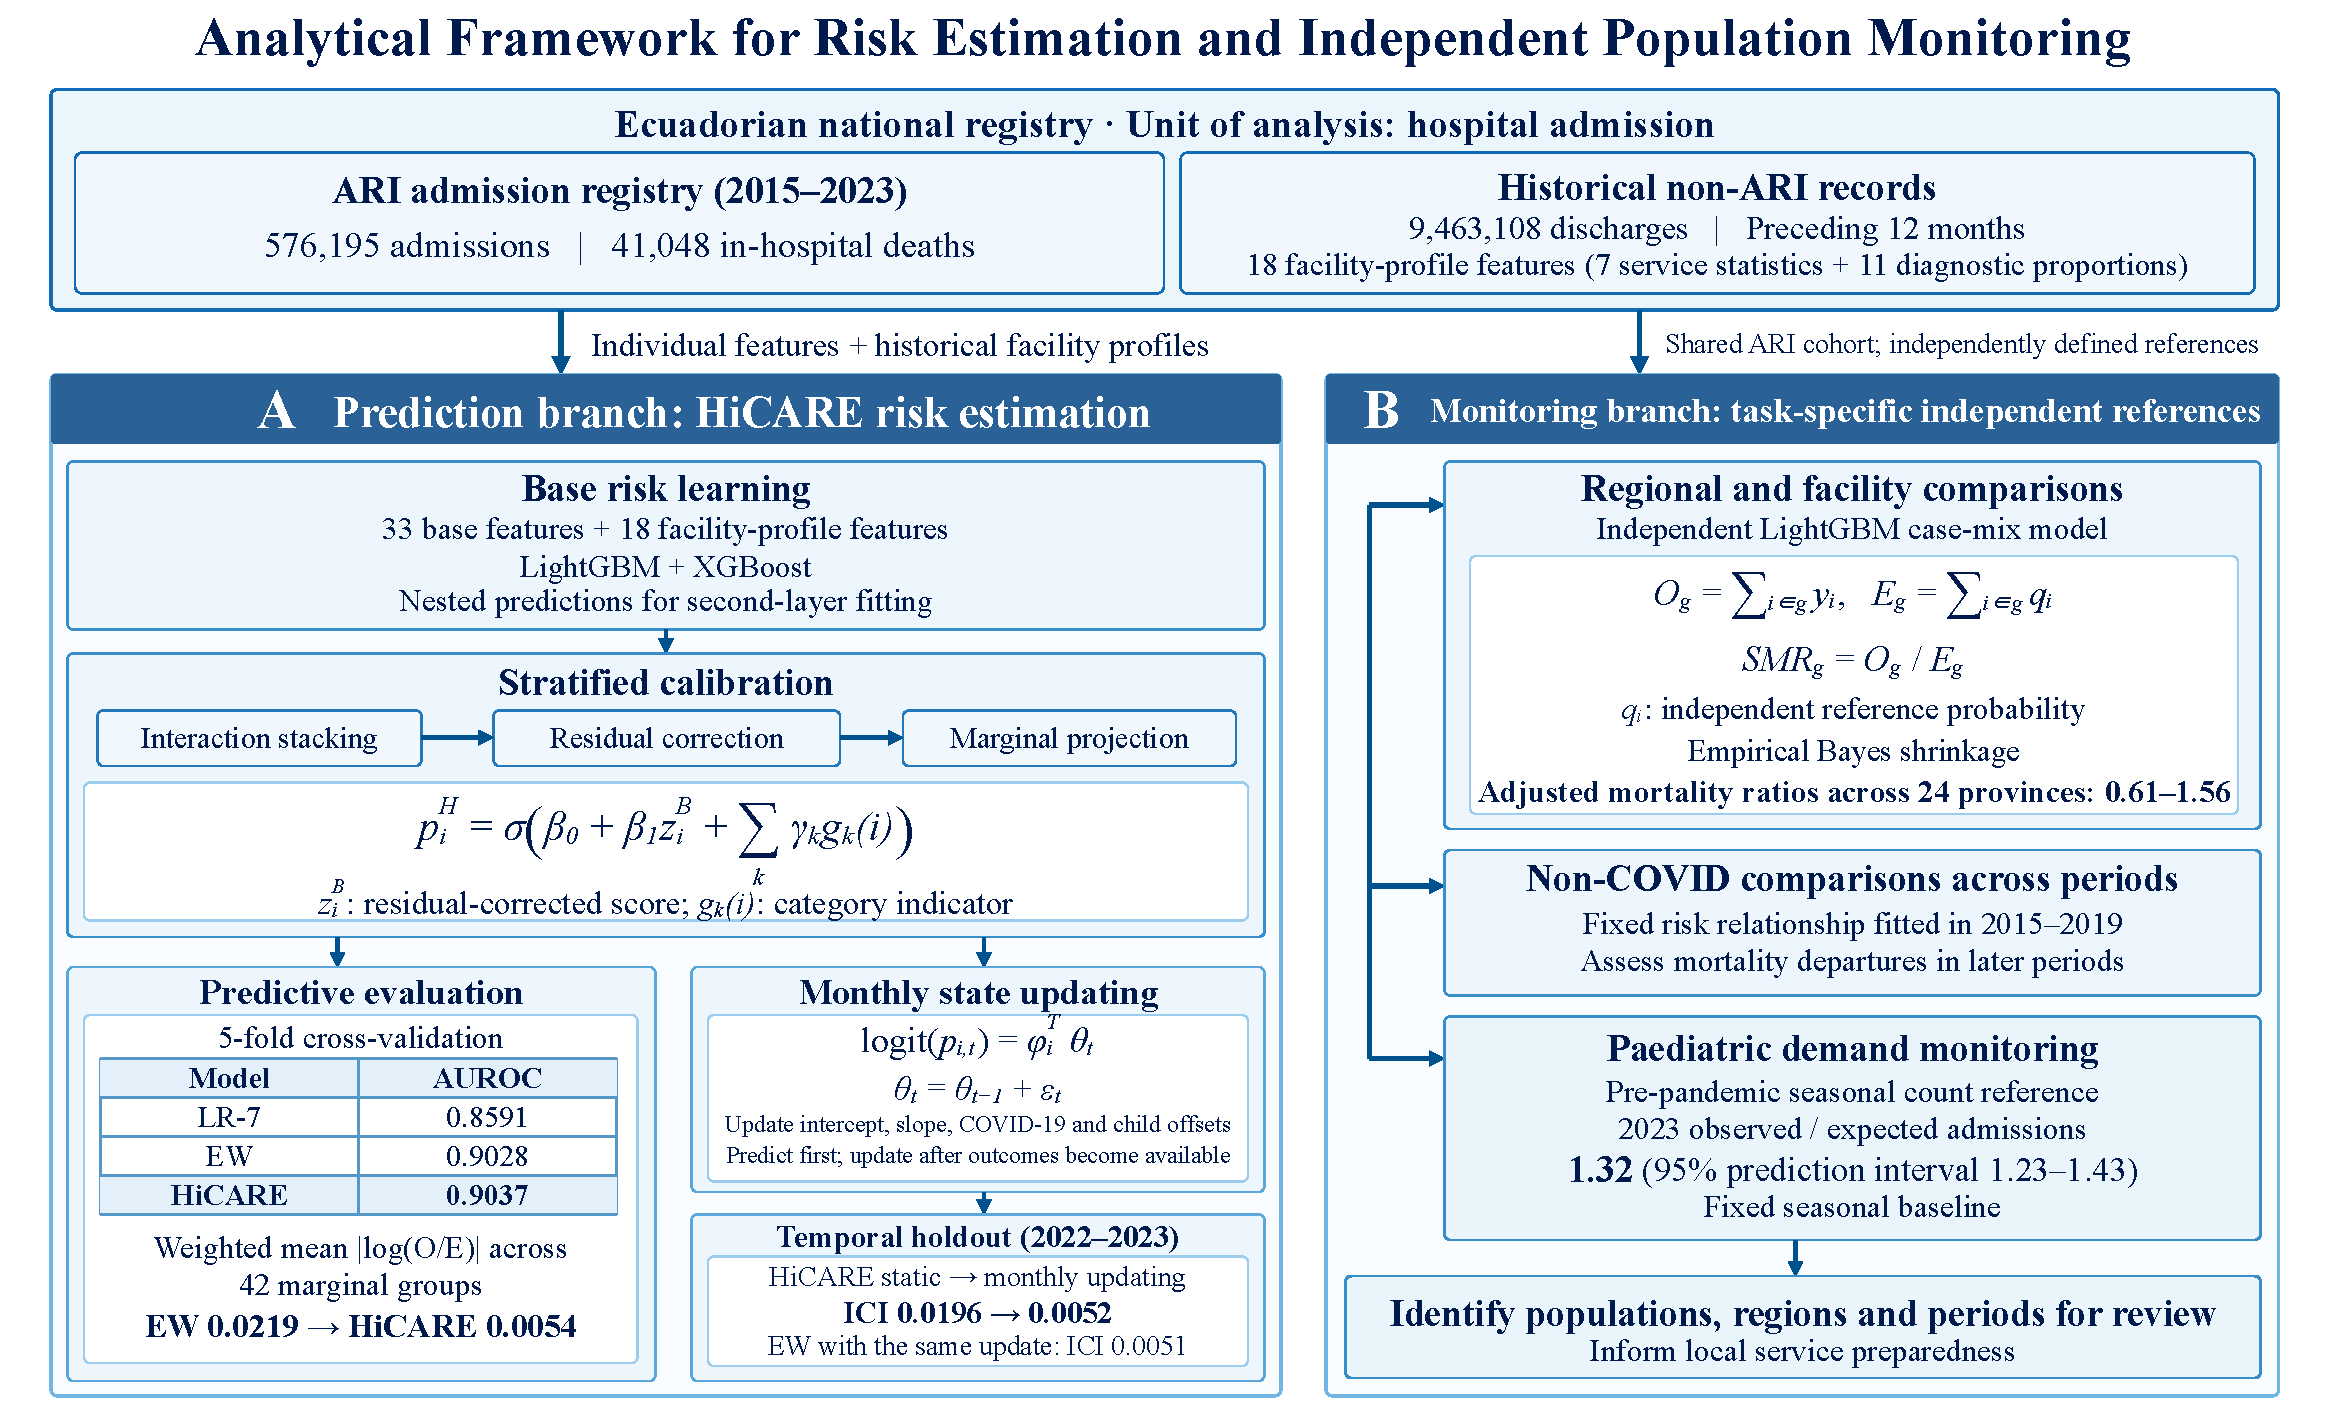
\includegraphics[width=\linewidth,height=173.925mm,keepaspectratio]{figures/risk_monitoring_supplied.pdf}
\captionof{figure}{Analytical framework for risk estimation and independent population monitoring. The shared registry contains 576,195 ARI admissions, including 41,048 in-hospital deaths; historical profiles draw on 9,463,108 non-ARI discharges. A, LightGBM and XGBoost predictions enter interaction stacking, residual correction and marginal projection, followed by monthly probability updating. Cross-validation and temporal holdout results summarise discrimination and calibration (Tables S4–S5). B, Independent references support regional and facility mortality comparisons, non-COVID historical comparisons and seasonal paediatric demand monitoring (Tables S7 and S13). Observed and expected deaths define the standardised mortality ratio; $q_i$ denotes an independent reference probability, not the HiCARE output. The branches share records but use different expected values. Provincial ratios and the paediatric prediction interval summarise monitoring results for further investigation.}\label{fig:arch}
\end{center}
For population g, observed deaths $O_g$ are the sum of outcomes, expected deaths $E_g$ are the sum of reference probabilities $q_i$, and the standardised mortality ratio (SMR) is $O_g$/$E_g$. Regional and facility $q_i$ values come from an independent LightGBM model restricted to variables such as age, sex, diagnosis and calendar background. Non-COVID period comparisons fix the 2015–2019 risk relationship, whereas paediatric demand uses pre-pandemic seasonal count models. These references assess differences between comparable cases, departures from historical relationships and changes in admission demand, respectively.

\begin{equation}
O_g=\sum_{i\in g}y_i,\quad E_g=\sum_{i\in g}q_i,\quad \mathrm{SMR}_g=O_g/E_g.
\end{equation}
The analyses share a registry cohort but not a common expected value. HiCARE discrimination and calibration measure predictive performance. Regional and temporal analyses using independent references describe observable outcome differences. The latter illustrate the decomposition of monitoring questions and do not directly demonstrate improved anomaly detection by HiCARE. Components and information sets are specified in Table S1 and Supplementary Section S1.

\clearpage
\subheading{3.3 Non-ARI records as historical facility service profiles}
Facility classes only coarsely describe admission roles. To capture differences in the populations actually served, we used 9,463,108 non-ARI discharges to summarise completed admissions in each facility group during the 12 months preceding the target month. The resulting 18 profile variables comprise seven service statistics and 11 diagnostic chapter proportions. They enter the base models alongside 33 individual and historical-context features.


\begin{center}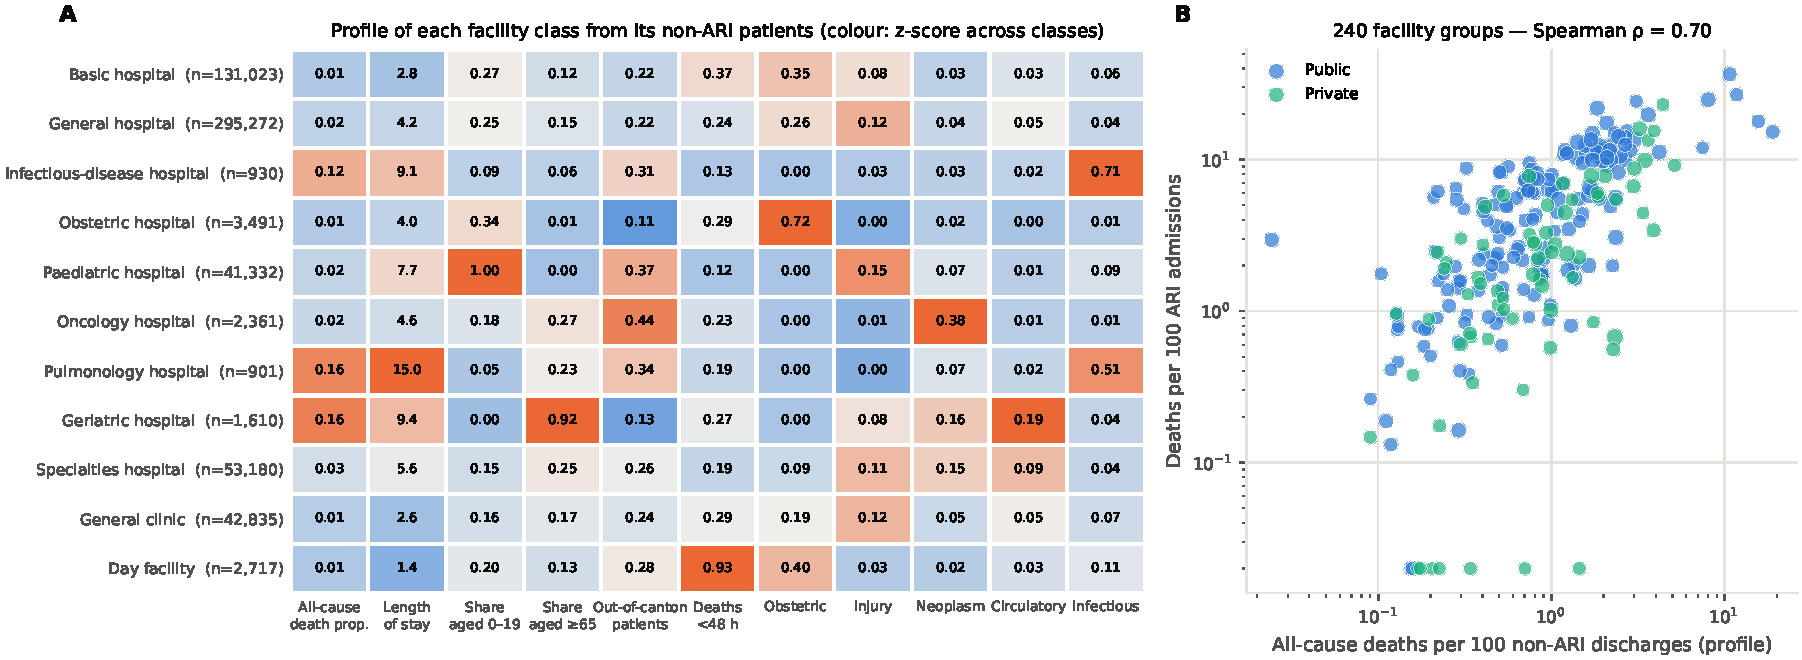
\includegraphics[width=\linewidth,height=167.725mm,keepaspectratio]{figures/x03_provider_profiles.pdf}
\captionof{figure}{Historical non-ARI service profiles. Left, Mean profiles by facility class. Right, Association between non-ARI all-cause and ARI mortality proportions across facility groups.}\label{fig:profiles}
\end{center}
Service statistics cover discharge volume, all-cause mortality, early-death composition, length of stay, age composition and cross-canton admission. Profiles require at least 30 historical records, with at least 10 deaths additionally required for early-death composition. A patient's own length of stay and post-discharge derived fields do not enter that patient's prediction features. Windows, missing-data handling and complete definitions are provided in Supplementary Section S1.

Age and diagnostic composition differ systematically between facilities, and non-ARI and ARI mortality proportions are associated. Profiles may therefore capture persistent case complexity and referral scope, supplementing sparse target records. However, they combine case selection and service context, and correlation alone cannot distinguish their clinical sources. Feature attribution and province-held-out evaluation examine whether the models use these inputs and how the corresponding configurations transfer.

\subheading{3.4 Stratified calibration, temporal updating and evaluation protocols}
Figure 3 details the learners, calibration stages and evaluation protocols underlying Figure 1A. LightGBM [34] and XGBoost [35] receive 33 base features and 18 facility-profile variables; panel A specifies their hyperparameters and early stopping. Clipped member probabilities become logit scores $z_i^{(m)}$, where m indexes learners. Stratified stacking lets the child indicator $c_i$ and COVID-19 indicator $v_i$ modify the intercept and member weights (Figure 3B, step 2a). Its expanded expression in the figure is equivalent to equation (2).

\begin{equation}
z_i^A=\alpha+bc_i+dv_i+\sum_m(a_m+b_mc_i+d_mv_i)z_i^{(m)}.
\end{equation}
\clearpage
The stratified score $z_i^A$ from equation (2) enters a shallow residual tree (Figure 3B, step 2b). The tree learns remaining deviations from specified variables $u_i$, including age, sex, ethnicity, facility, region and month, to obtain a corrected score.

\begin{equation}
z_i^B=z_i^A+h(u_i,z_i^A).
\end{equation}
Residual correction minimises record-level loss, whereas accurate group totals require a further calibration step. An unpenalised logistic projection combines $z_i^B$ with marginal-category indicators $g_k(i)$ to obtain the HiCARE probability (Figure 3B, step 2c).

\begin{equation}
p_i^H=\sigma\!\left(\beta_0+\beta_1z_i^B+\sum_k\gamma_kg_k(i)\right).
\end{equation}
Here, $\sigma$ is the logistic function. The $g_k$ indicators cover age, sex, ethnicity, residence area, sector and infection type; year is also included in the within-distribution configuration. Category residual sums approach zero in the projection fitting sample when a finite solution exists and optimisation converges, but held-out groups require separate evaluation. Parameters are summarised in Figure 3B and score equations in Supplementary Section S1.

Temporal maintenance forms a four-dimensional input from $z_i^H$=logit($p_i^H$), representing the intercept, score slope and two population offsets by monthly state $\theta_t$ (Figure 3C).

\begin{equation}
\phi_i=[1,z_i^H,v_i,c_i]^\top,\quad \operatorname{logit}(p_{i,t})=\phi_i^\top\theta_t.
\end{equation}
\begin{equation}
\theta_t=\theta_{t-1}+\varepsilon_t,\quad \varepsilon_t\sim N(0,qI),\quad q=0.1.
\end{equation}
I is the four-dimensional identity matrix. Each month is predicted using the previous month's state, followed by a Laplace update when outcomes become available. Four state coefficients and q=0.1 were selected by forward-validation log loss during 2018–2021 (Table S2). Development used 2015–2021 and testing used 2022–2023, comparing static, rolling and identically state-updated models. The retrospective simulation did not strictly incorporate reporting delay.

Within-distribution evaluation uses five stratified outer folds. In each training partition, four inner splits rotate three fitting folds and one prediction fold, giving 20 outer–inner combinations per learner (Figure 3D). Nested predictions train the second layer, evaluated on the outer holdout. Fifteen per cent of second-layer records support residual-tree early stopping; projection uses all records. Historical statistics are precomputed, so direct training separation does not ensure complete historical-information isolation.

Geographic transfer uses six province-grouped folds with geographic identifiers removed and evaluates only profile-ensemble configurations. The configuration without profiles contains LightGBM, XGBoost and TabM; the profile configuration contains the first two and does not run the full second layer. Local historical data remain available at test time, and precomputed context may contain past outcomes from held-out provinces. Differences therefore involve profiles, learner composition and available history together.

Comparators are seven-variable logistic regression (LR-7) and an equal-weight ensemble of three learners (EW; Figure 3E). LR-7 includes age group, sex, ethnicity, residence area, public/private sector, infection type and year. Historical figure labels 'Reference LR' or 'Reference model' denote LR-7, and 'CARE v1' denotes EW. AUROC and AUPRC, computed as average precision, measure discrimination. Log loss and the Brier score assess probability error. ICI, sample-size-weighted mean and maximum |log(O/E)| across 42 marginal groups, and worst eligible-group ECE assess overall calibration, group totals and within-group error.

Primary results use random seed 0 and record-level paired bootstrap resampling. Temporal LR-7 is selected post hoc from nine variants by test loss. Decision curves and death coverage describe retrospective screening under hypothetical rules. Metric definitions and eligibility thresholds are given in Supplementary Section S1 and Tables S3–S6.

\clearpage

\begin{center}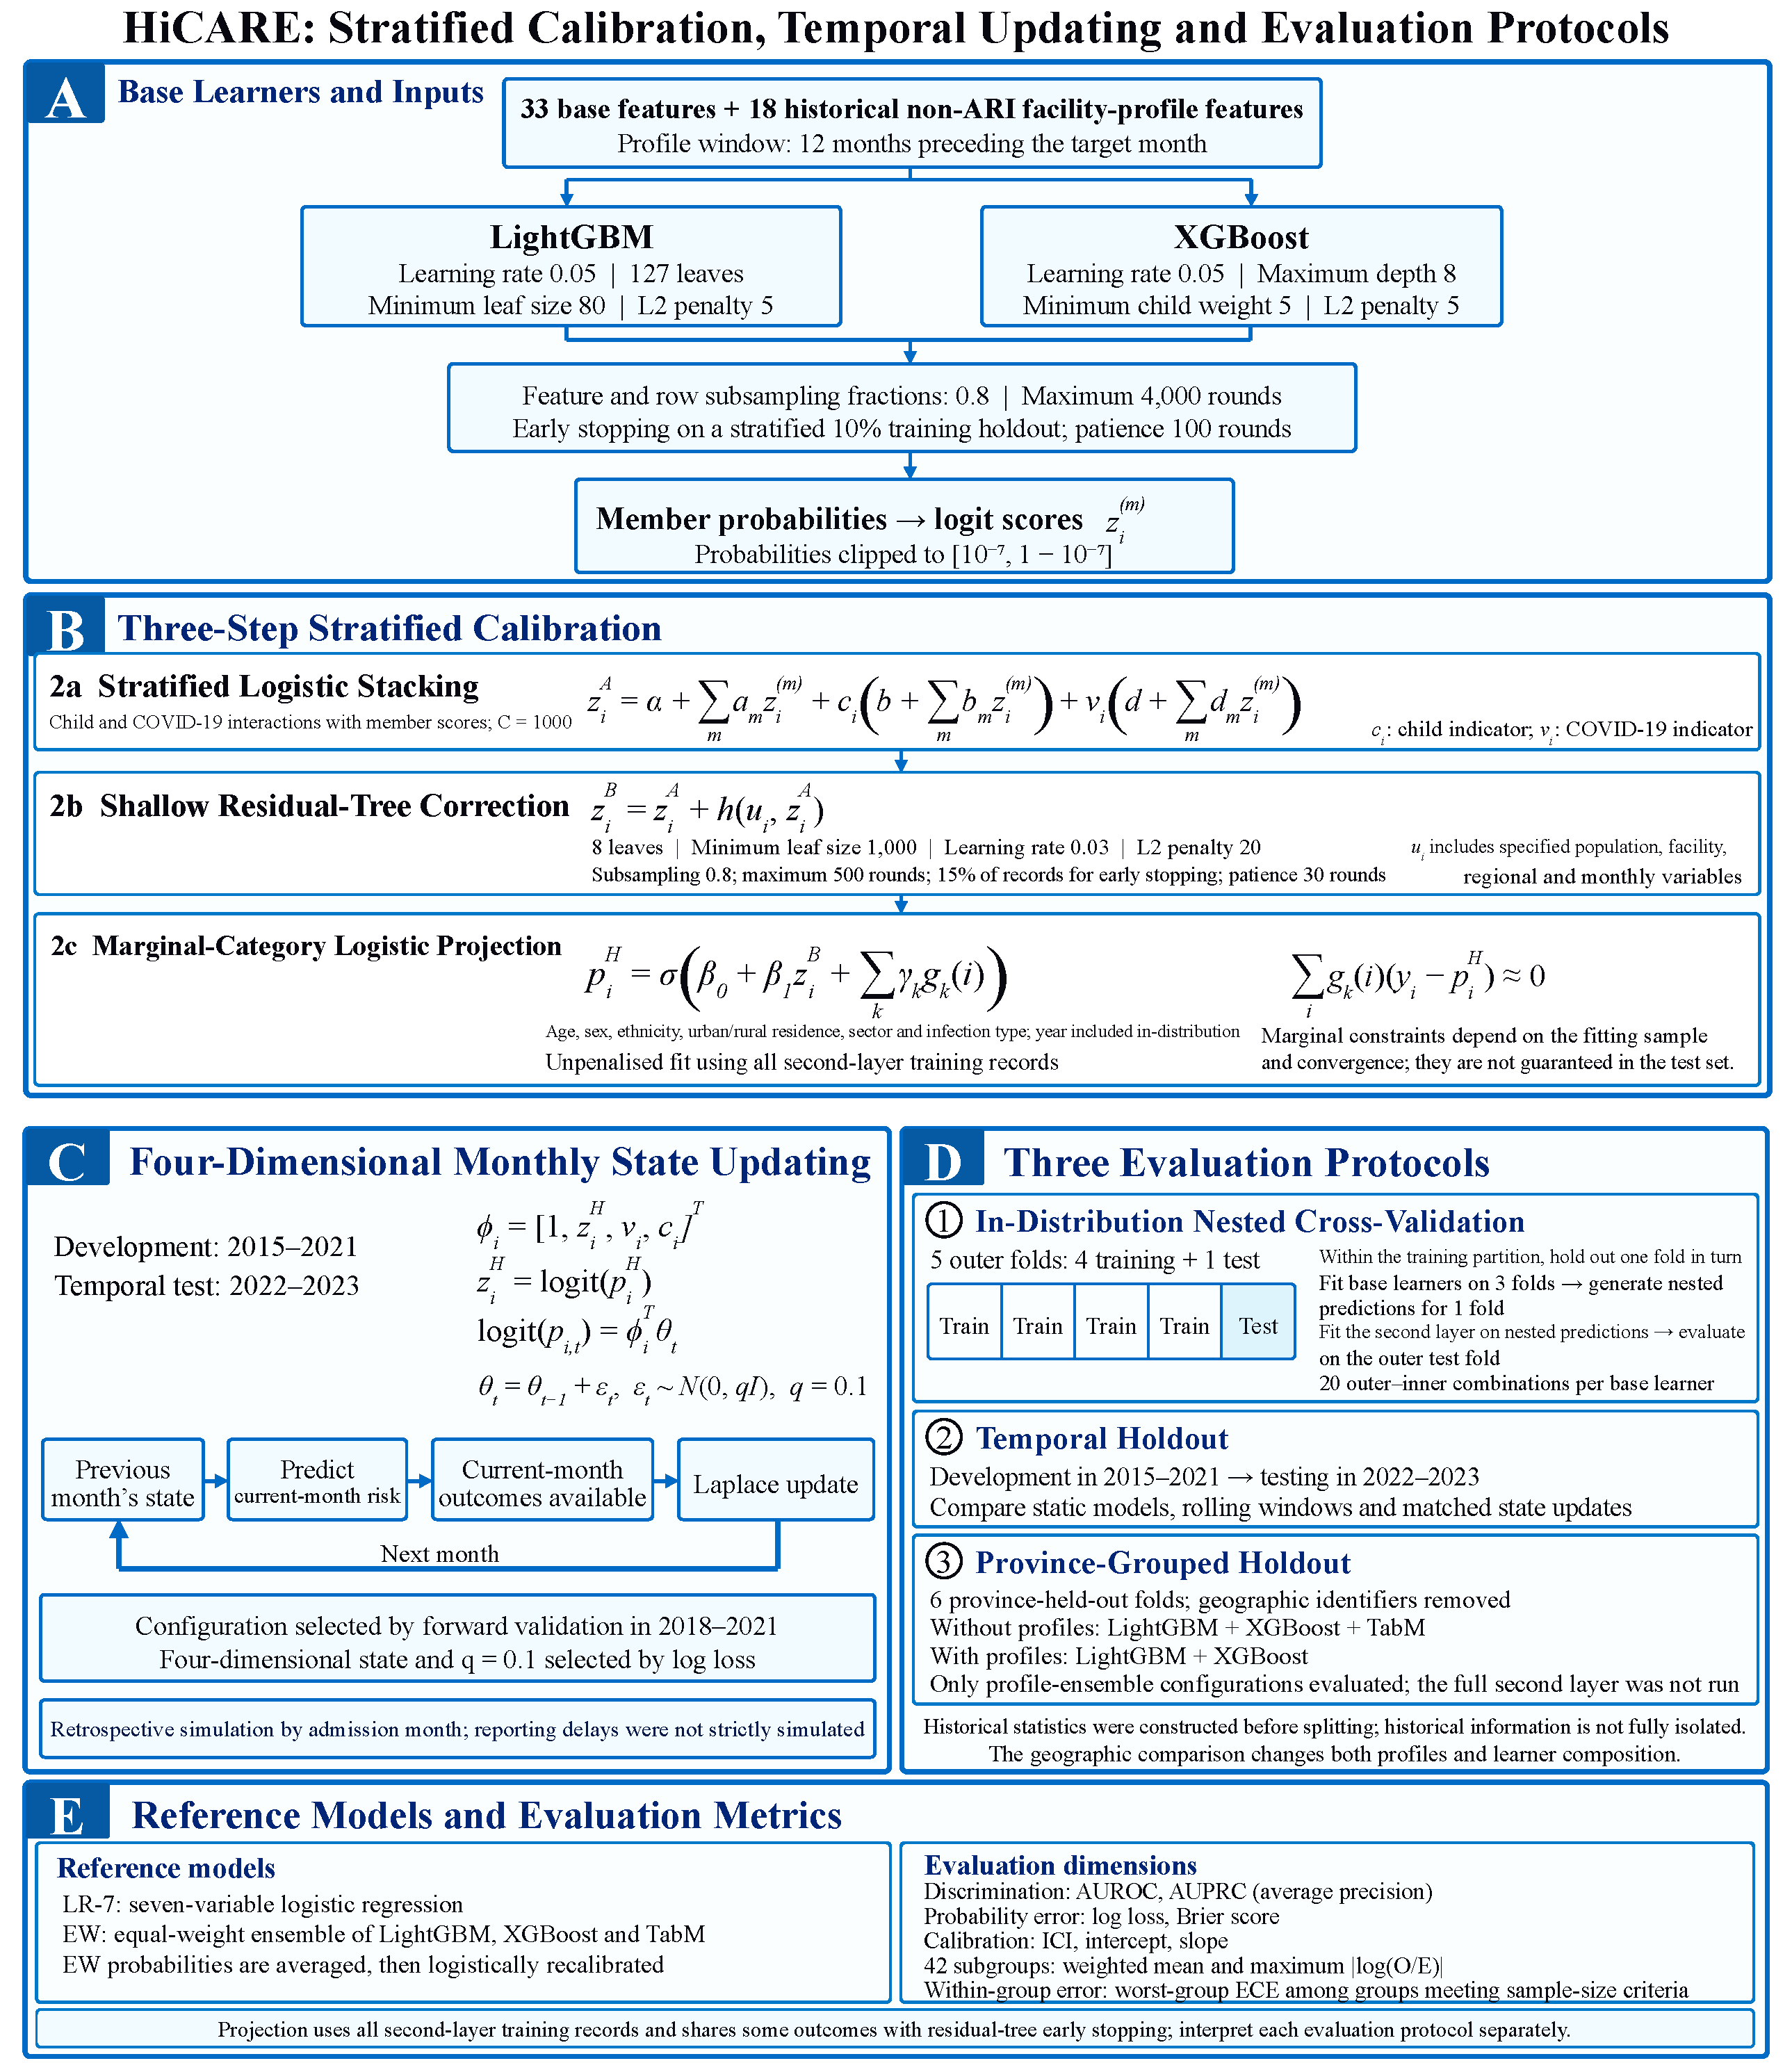
\includegraphics[width=\linewidth,height=205mm,keepaspectratio]{figures/hicare_methods_supplied.pdf}
\captionof{figure}{HiCARE stratified calibration, temporal updating and evaluation protocols. A, Base features, historical profiles, LightGBM and XGBoost hyperparameters, and conversion of member probabilities to logit scores. B, Three calibration stages comprise stratified stacking (2a), residual-tree correction (2b) and marginal logistic projection (2c), corresponding to equations (2)–(4). C, Four-dimensional monthly states and the predict-then-update cycle, corresponding to equations (5)–(6). D, Nested cross-validation, temporal holdout and province-grouped holdout; the province protocol evaluates profile ensembles without the full second layer. E, Reference models and evaluation metrics. The indicators $c_i$ and $v_i$ identify children and COVID-19, m indexes learners, and $g_k$ identifies marginal categories. Historical summaries are precomputed, and projection shares outcomes with residual early stopping. The marginal constraint applies to fitting data and does not guarantee calibration in held-out populations.}\label{fig:hicare_detailed}
\end{center}
\clearpage
\mainheading{4 Results}
\subheading{4.1 Ranking improves within both age strata}
HiCARE improved on LR-7 within children and adults, rather than merely separating populations with very different baseline mortality. All-age AUROC increased from 0.859 to 0.904 and log loss fell from 0.1934 to 0.1701. Paediatric AUROC increased from 0.689 to 0.874 and adult AUROC from 0.729 to 0.817 (Table S3). Figure 4 shows the corresponding performance across screening thresholds.


\begin{center}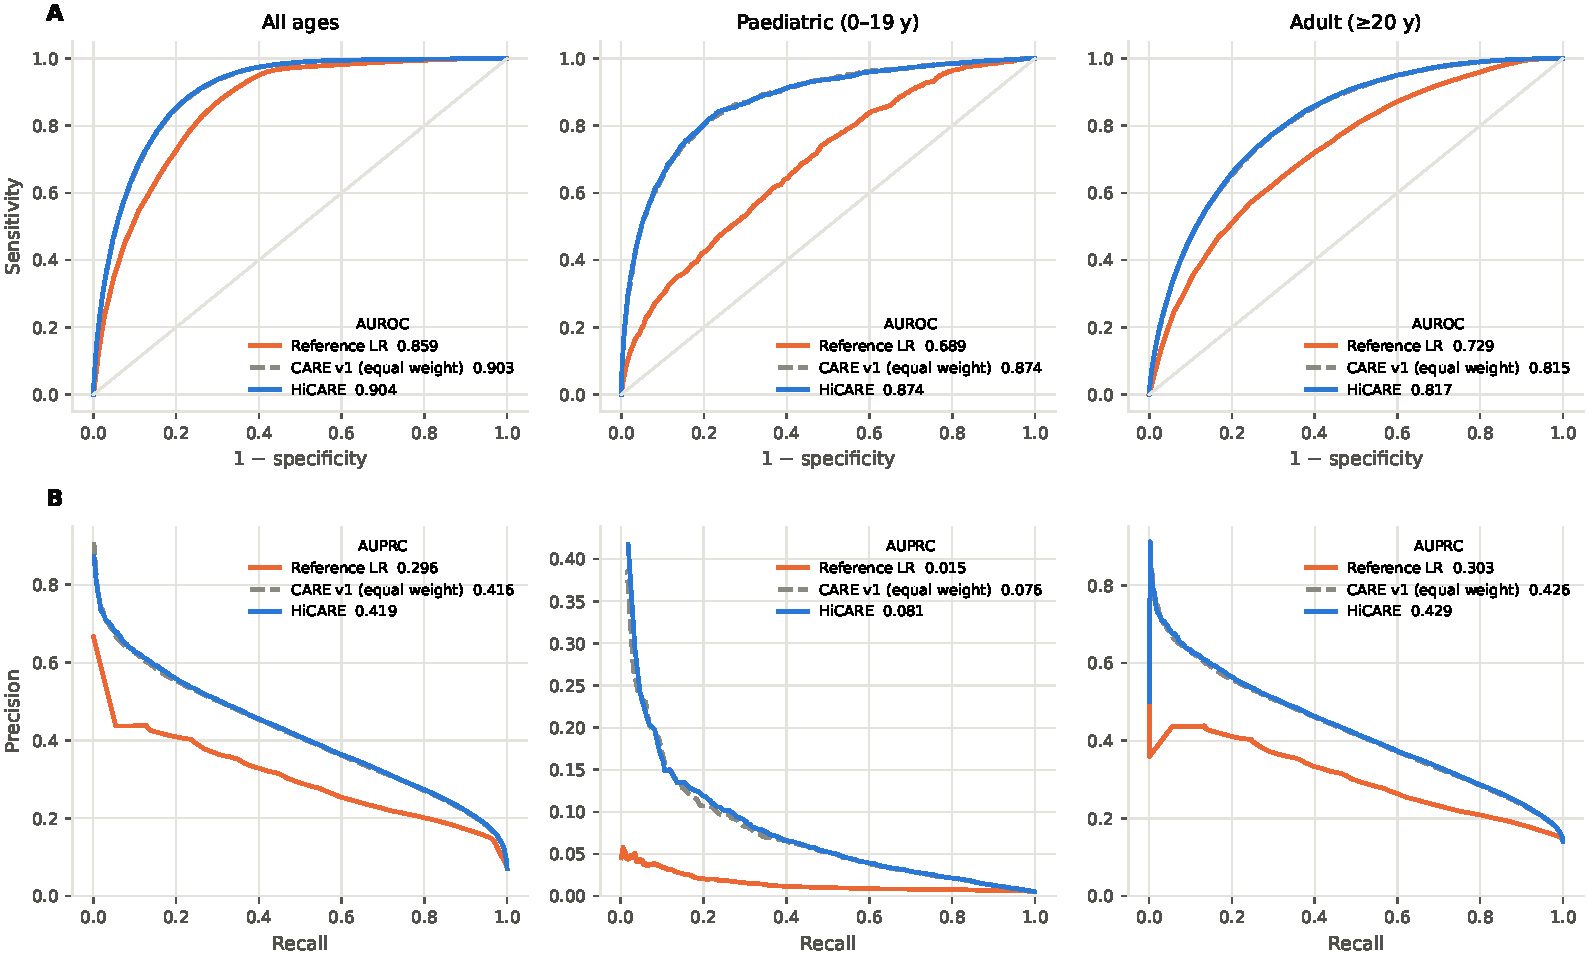
\includegraphics[width=\linewidth,height=193.225mm,keepaspectratio]{figures/x04_roc_pr.pdf}
\captionof{figure}{Cross-validated (A) receiver operating characteristic and (B) precision–recall curves.}\label{fig:rocpr}
\end{center}
Paediatric deaths were rare, making precision–recall curves particularly informative about the difficulty of identifying deaths among many surviving admissions. Paediatric AUPRC increased from 0.015 with LR-7 to 0.081 with HiCARE, indicating a greater concentration of deaths near the top of the risk ranking. The absolute value nevertheless remained low. Review volume therefore remains a trade-off against mortality coverage; improved ranking does not imply that a small review sample can capture all deaths.

The HiCARE and EW curves largely overlapped, with EW already achieving an all-age AUROC of 0.903. The base ensemble thus provided most of the discrimination. The additional calibration layer should instead be assessed by whether it changes the allocation of probabilities while preserving that ranking. We therefore examined individual probability errors and aggregated expected deaths.

\clearpage
\subheading{4.2 Probability accuracy and screening value provide complementary evidence}

\begin{center}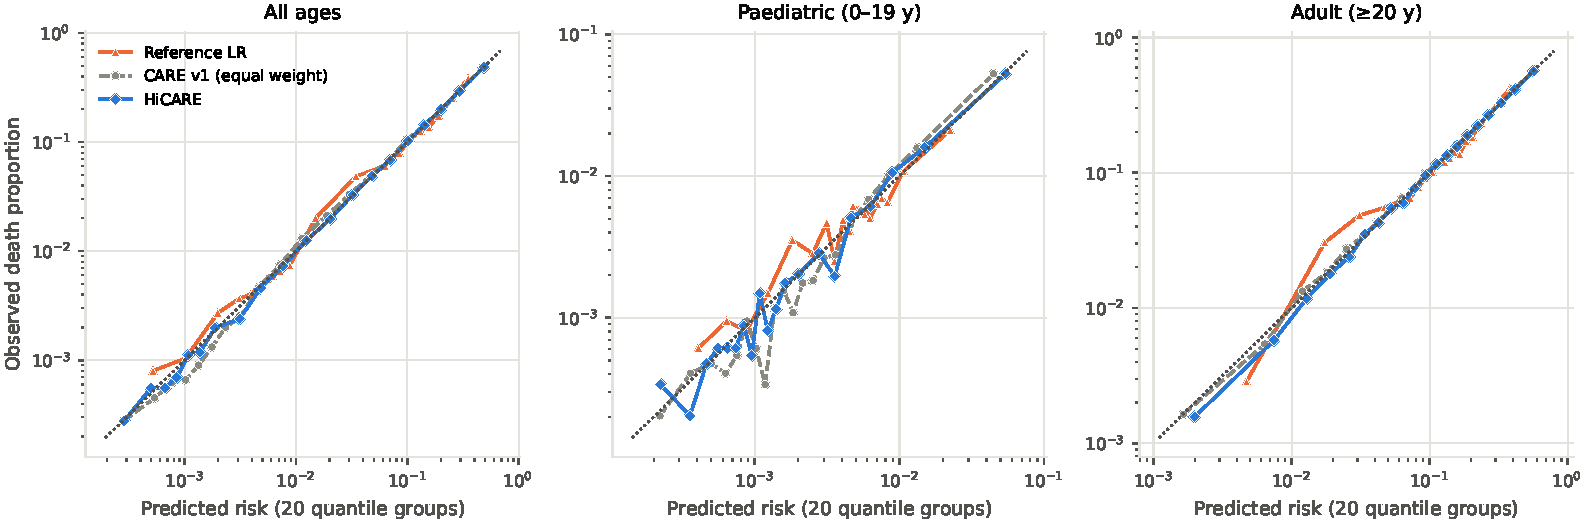
\includegraphics[width=\linewidth,height=94.9025mm,keepaspectratio]{figures/x05_calibration.pdf}
\captionof{figure}{Age-specific calibration curves. Curves use 20 predicted-risk quantile bins on logarithmic axes; tabulated ICI values use an isotonic approximation with 200 bins.}\label{fig:calib}
\end{center}
HiCARE predictions tracked observed frequencies in both low-risk children and adults spanning a broader risk range (Figure 5). ICI was 0.0006 in children and 0.0033 in adults. The lower absolute error in children partly reflects their lower baseline mortality. It should therefore be interpreted alongside the low-probability calibration curve and AUPRC, rather than as evidence that paediatric risk is easier to predict.


\begin{center}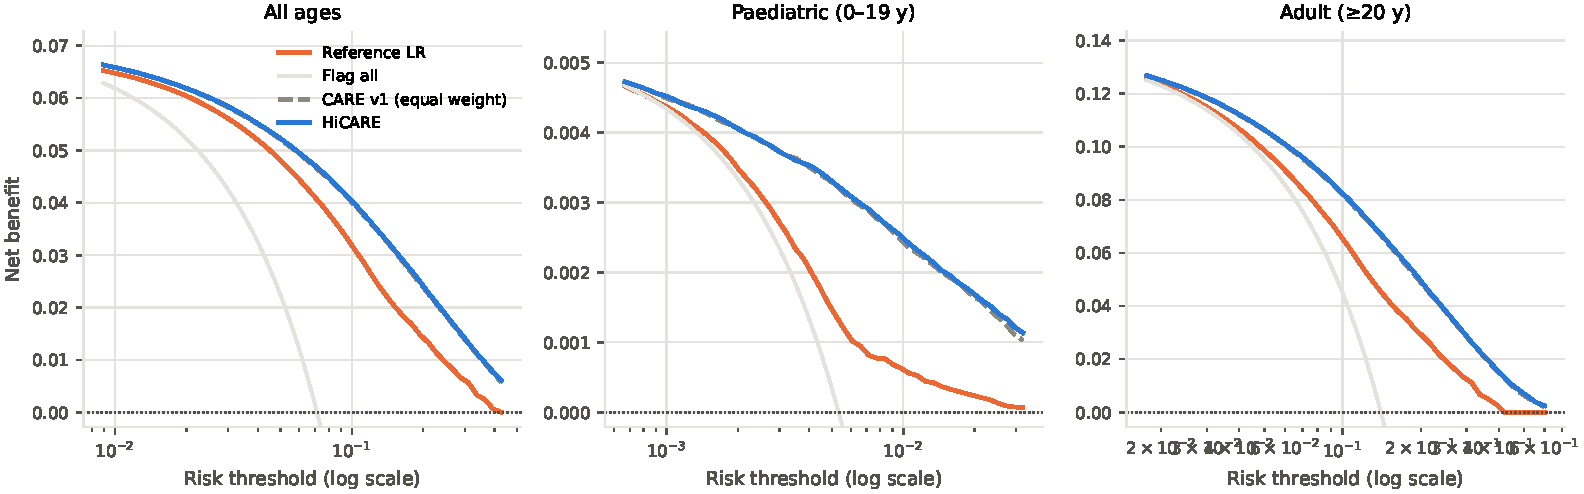
\includegraphics[width=\linewidth,height=94.9025mm,keepaspectratio]{figures/x06_decision_curves.pdf}
\captionof{figure}{Decision curves in cross-validation.}\label{fig:dca}
\end{center}
Across the displayed thresholds, HiCARE and EW had similar net benefit and generally exceeded LR-7 (Figure 6). Better ranking therefore translated into potential screening value under the assumed false-positive costs, although HiCARE did not show a large decision advantage over EW. Together, these results show that baseline risk identification was already strong. The contribution of the subsequent calibration steps must be assessed against the group-level errors they target.

\clearpage
\subheading{4.3 Stratified calibration primarily improves group-level predicted totals}
After adding facility profiles, the equal-weight configuration achieved an AUROC of 0.9033, while mean absolute log(O/E) across the specified subgroups remained 0.0229. Stratified stacking, residual correction and marginal projection successively reduced this error to 0.0126, 0.0089 and 0.0054, with AUROC varying only between 0.9035 and 0.9037 (Table S4). Figure 7 therefore supports a specific interpretation. The calibration steps primarily redistributed probabilities within a similar risk ranking, bringing aggregated expected deaths closer to observed counts.


\begin{center}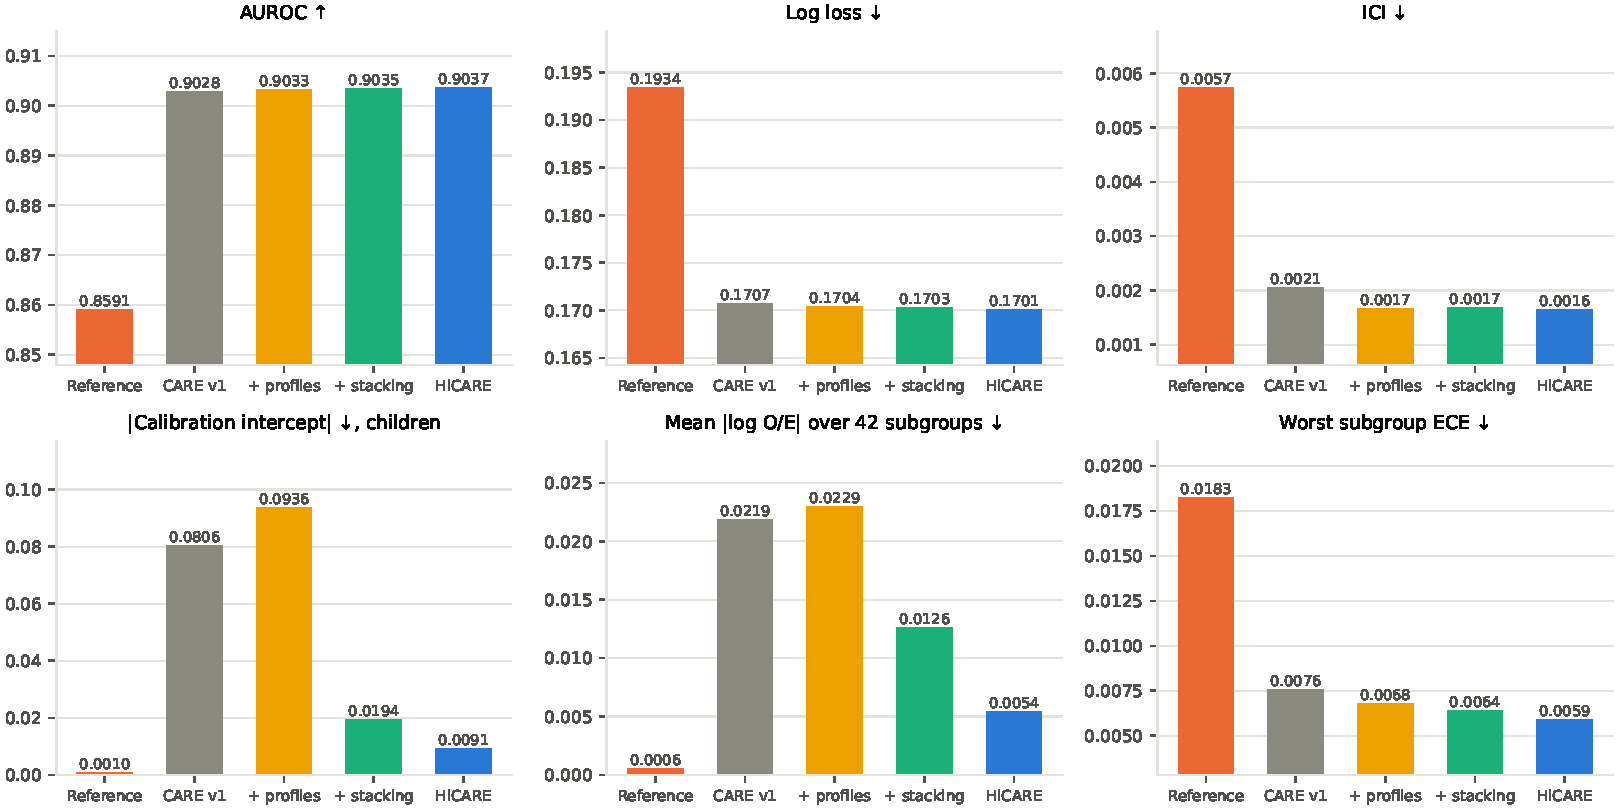
\includegraphics[width=\linewidth,height=189.505mm,keepaspectratio]{figures/t2_layer_contributions.pdf}
\captionof{figure}{Contributions of facility profiles and components of the second calibration layer in cross-validation.}\label{fig:layers}
\end{center}
Relative to the original EW model, the point estimate of mean marginal error fell by 75.3\%, whereas AUROC increased by only 0.0009. This distinction clarifies the roles of the model components and prevents the overall advantage over LR-7 from being attributed entirely to the second layer. A single-LightGBM configuration also achieved an AUROC of 0.9037 and a log loss of 0.1701, indicating that a complex ensemble was not required to retain most of the predictive performance.

Marginal projection introduced an interpretable trade-off. Maximum absolute log(O/E) decreased from 0.166 to 0.076, but worst-group ECE increased from 0.0050 to 0.0059. The former measures whole-group totals, whereas the latter measures errors within risk intervals. Improving group totals can still allow local overprediction and underprediction to cancel. Both checks are therefore needed when selecting a model.

\clearpage

\begin{center}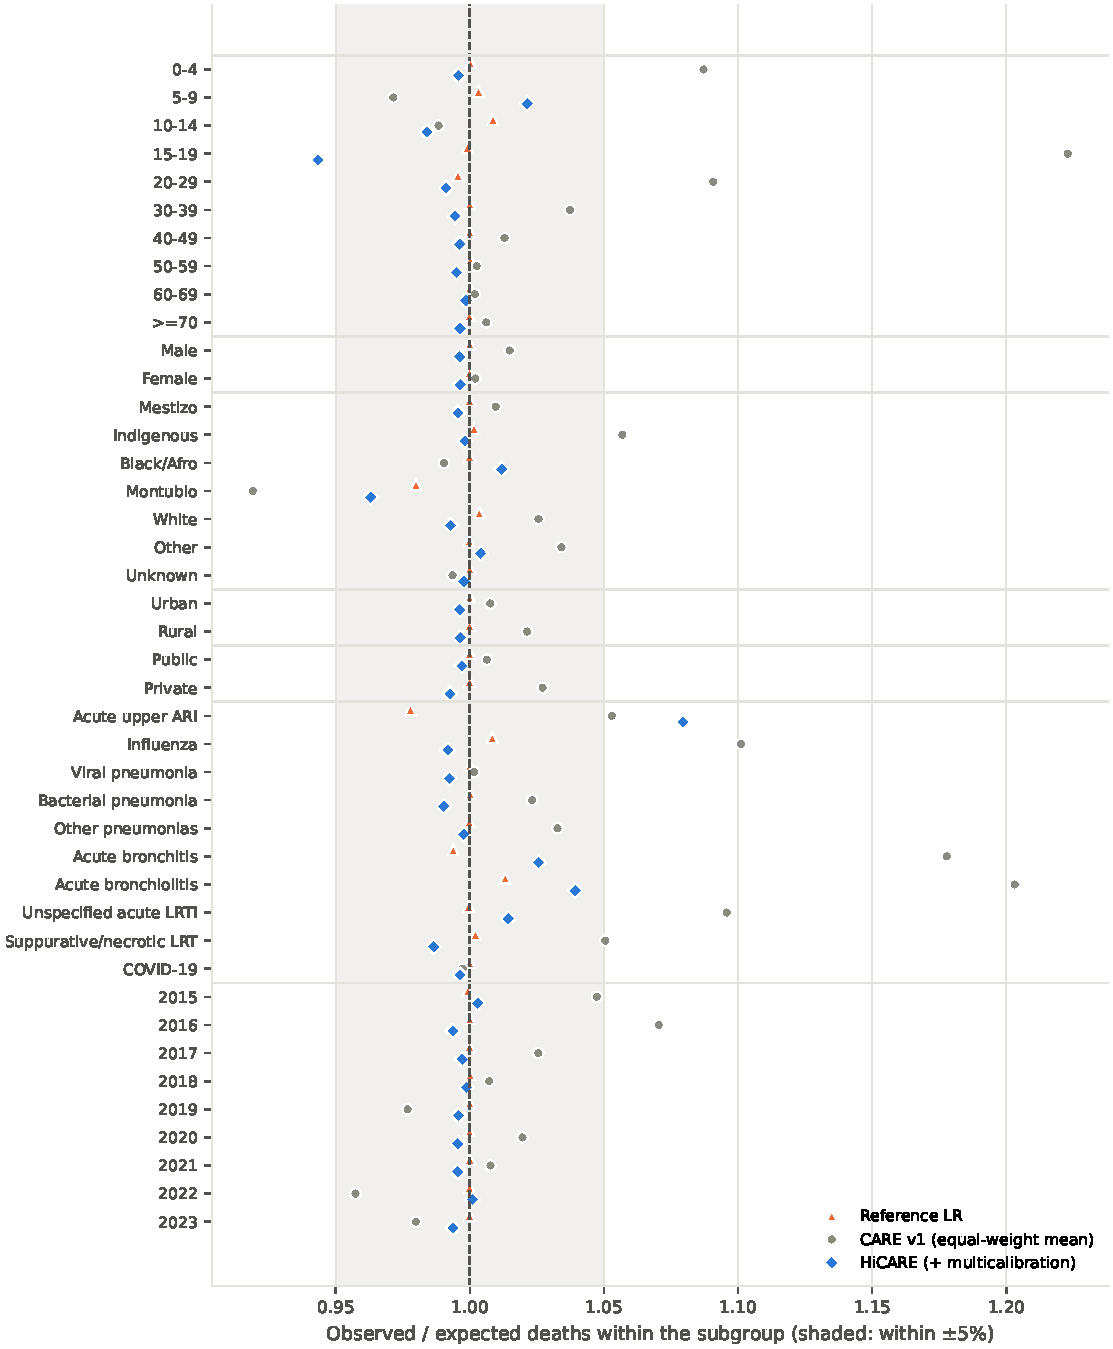
\includegraphics[width=\linewidth,height=195mm,keepaspectratio]{figures/t1_subgroup_calibration.pdf}
\captionof{figure}{Observed-to-expected mortality ratios in 42 specified marginal groups. The legacy label “+ multicalibration” denotes residual correction and marginal projection here; it does not imply guaranteed calibration in arbitrary intersecting populations.}\label{fig:subcal}
\end{center}
Disaggregating the mean error showed that HiCARE reduced the largest departures in group O/E relative to EW (Figure 8). The groups covered age, sex, ethnicity, urban or rural residence, sector, infection type and year, matching the populations for which monitoring totals were intended. These findings support correction within specified marginal categories, rather than an inference that accurate overall probabilities ensure accuracy in every population.

LR-7 also had a small mean marginal error of 0.0006, but its worst-group ECE was 0.0183, compared with 0.0059 for HiCARE (Table S4). Accurate group means and informative within-group risk estimates can therefore diverge. HiCARE retained strong risk identification while reducing conspicuous errors in predicted totals for the specified populations.

\clearpage
\subheading{4.4 Direction of improvement and use of facility information}

\begin{center}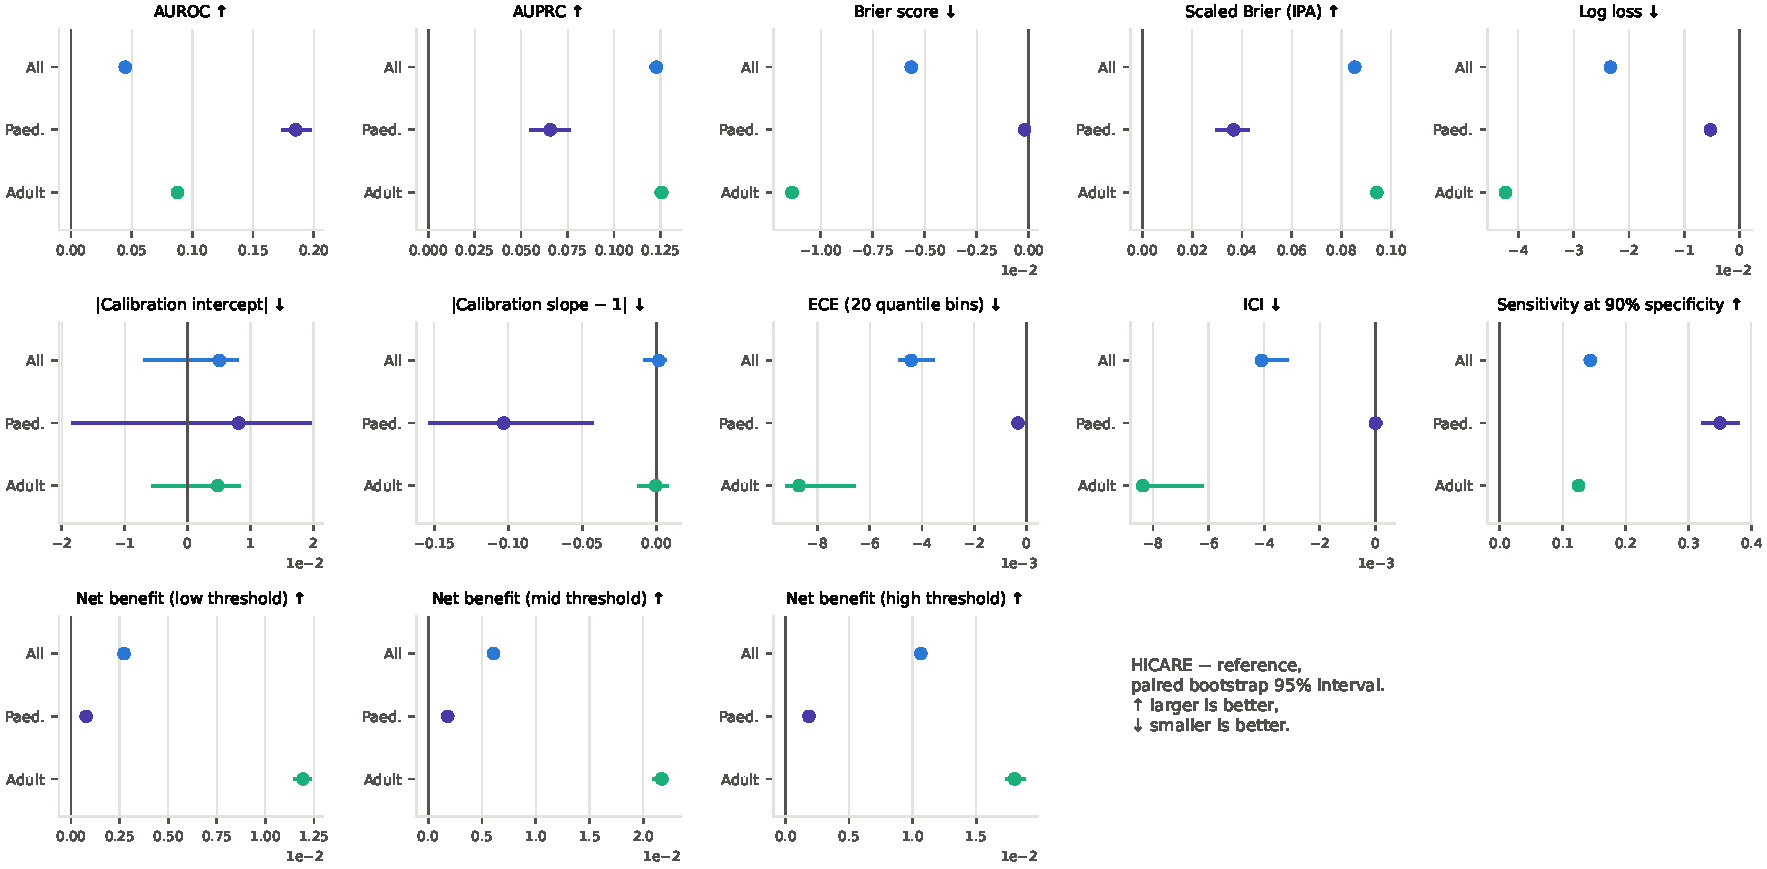
\includegraphics[width=\linewidth,height=93.5075mm,keepaspectratio]{figures/x08_bootstrap_forest.pdf}
\captionof{figure}{Paired bootstrap differences between HiCARE and LR-7. The favourable direction depends on the metric; intervals are based on resampling admission records.}\label{fig:boot}
\end{center}
AUROC and AUPRC difference intervals lay above zero in all-age, paediatric and adult evaluations, whereas log-loss differences lay below zero (Figure 9). The paediatric ICI difference was close to zero. In children with low baseline mortality, the model primarily improved ranking without a comparably large change in mean absolute probability error, consistent with the separate discrimination and calibration assessments.


\begin{center}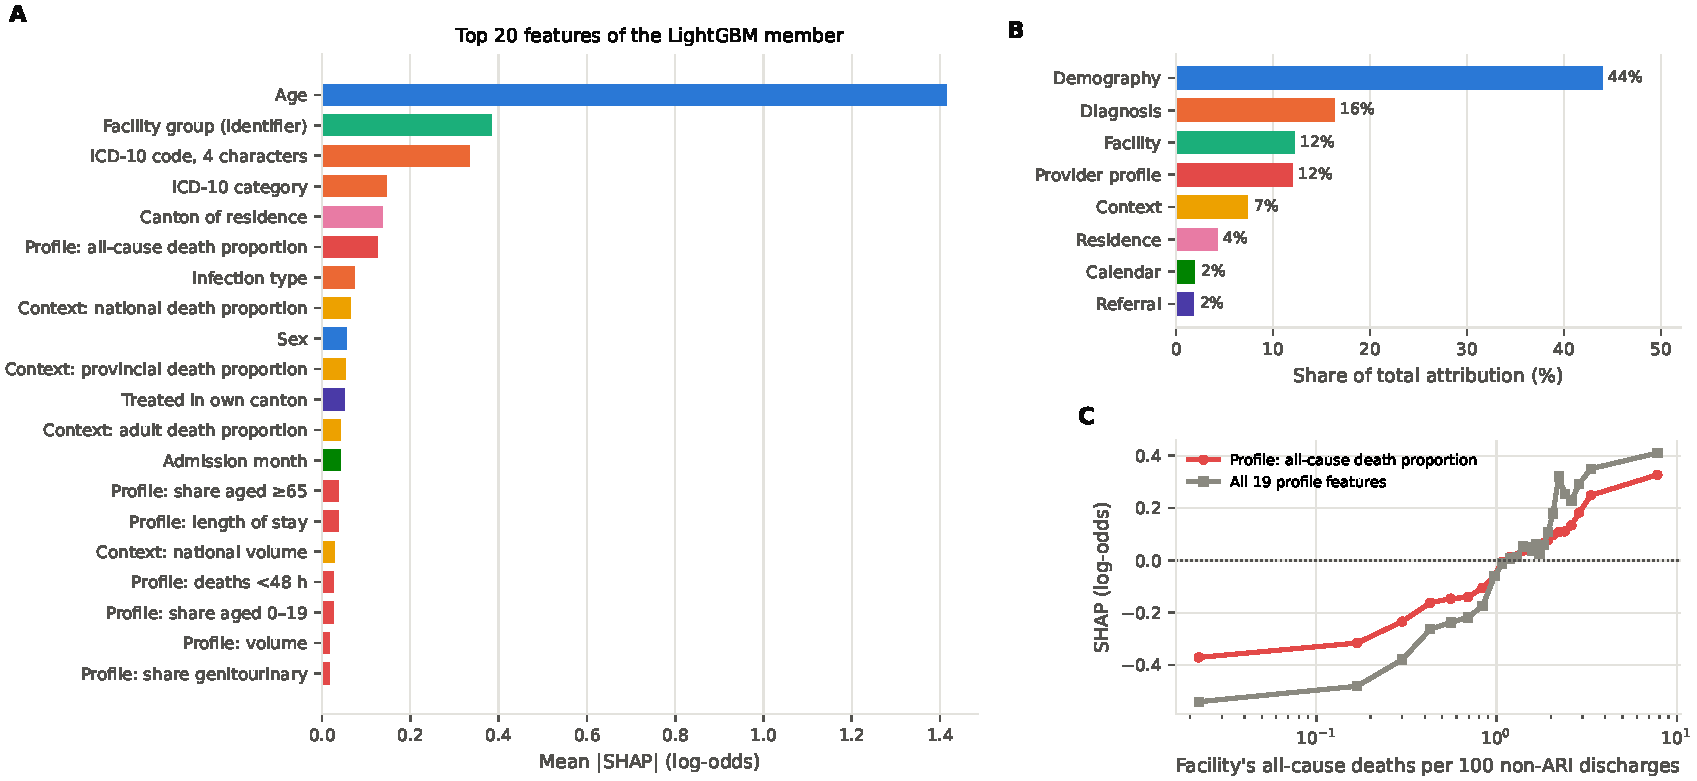
\includegraphics[width=\linewidth,height=93.5075mm,keepaspectratio]{figures/x10_shap_profiles.pdf}
\captionof{figure}{TreeSHAP attribution for the base tree model. Panels show leading features, attribution shares by feature group and the relationship between historical facility non-ARI mortality and attribution.}\label{fig:shapv2}
\end{center}
Shapley additive explanations (SHAP) assigned approximately 12\% of total attribution to facility profiles, and non-ARI mortality was among the leading features (Figure 10). The fitted model therefore used historical information beyond the target disease. Attribution shares describe how a model allocates its scores; they neither quantify the performance gain from profiles nor identify historical mortality as a measure of facility quality. Transferability must be assessed in held-out regions.

\clearpage
\subheading{4.5 Temporal change primarily requires maintenance of the probability scale}

\begin{center}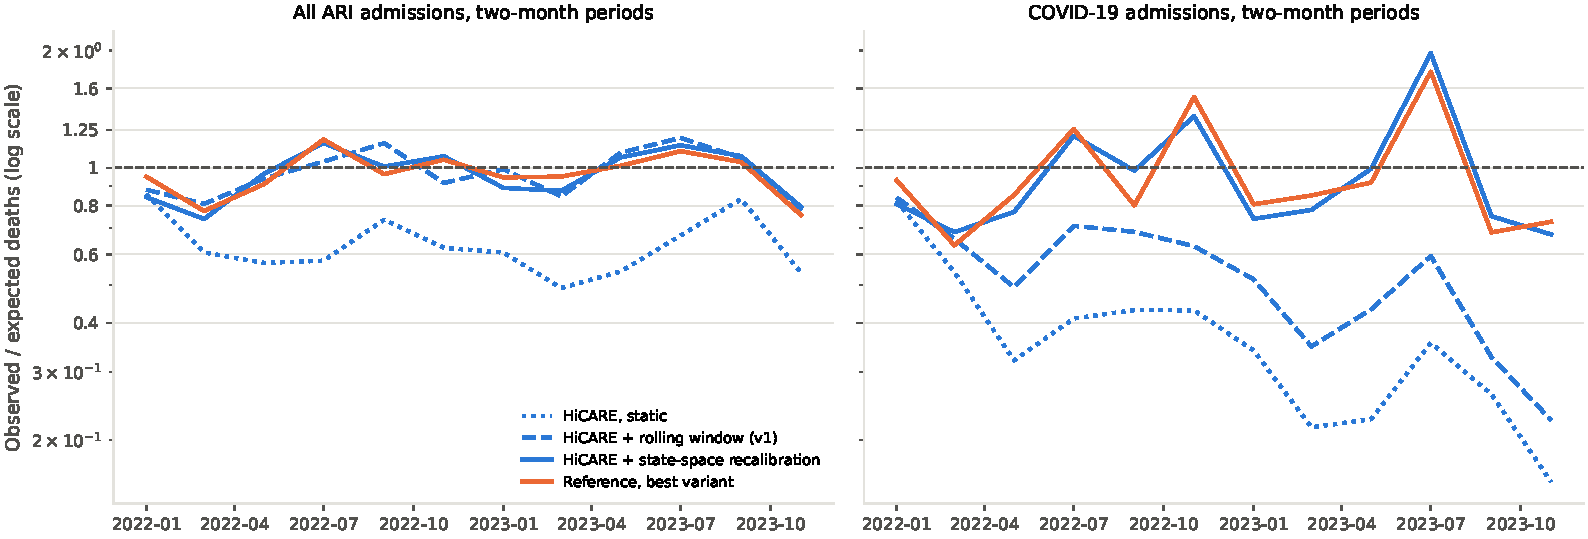
\includegraphics[width=\linewidth,height=92.655mm,keepaspectratio]{figures/t3_dynamic_recalibration.pdf}
\captionof{figure}{Bimonthly O/E in 2022–2023 under static prediction, rolling windows and state updating. The best LR-7 variant was selected retrospectively by test-set loss.}\label{fig:dyn}
\end{center}
Static HiCARE had an O/E of 0.66, indicating sustained overprediction of subsequent mortality. State updating increased O/E to 0.93, reduced ICI from 0.0196 to 0.0052 and reduced log loss from 0.1220 to 0.1163, while AUROC changed only from 0.899 to 0.900 (Table S5; Figure 11). EW achieved the same log loss of 0.1163 with identical updating. The principal benefit in this setting thus arose from probability maintenance rather than a uniquely advantageous complex architecture.


\begin{center}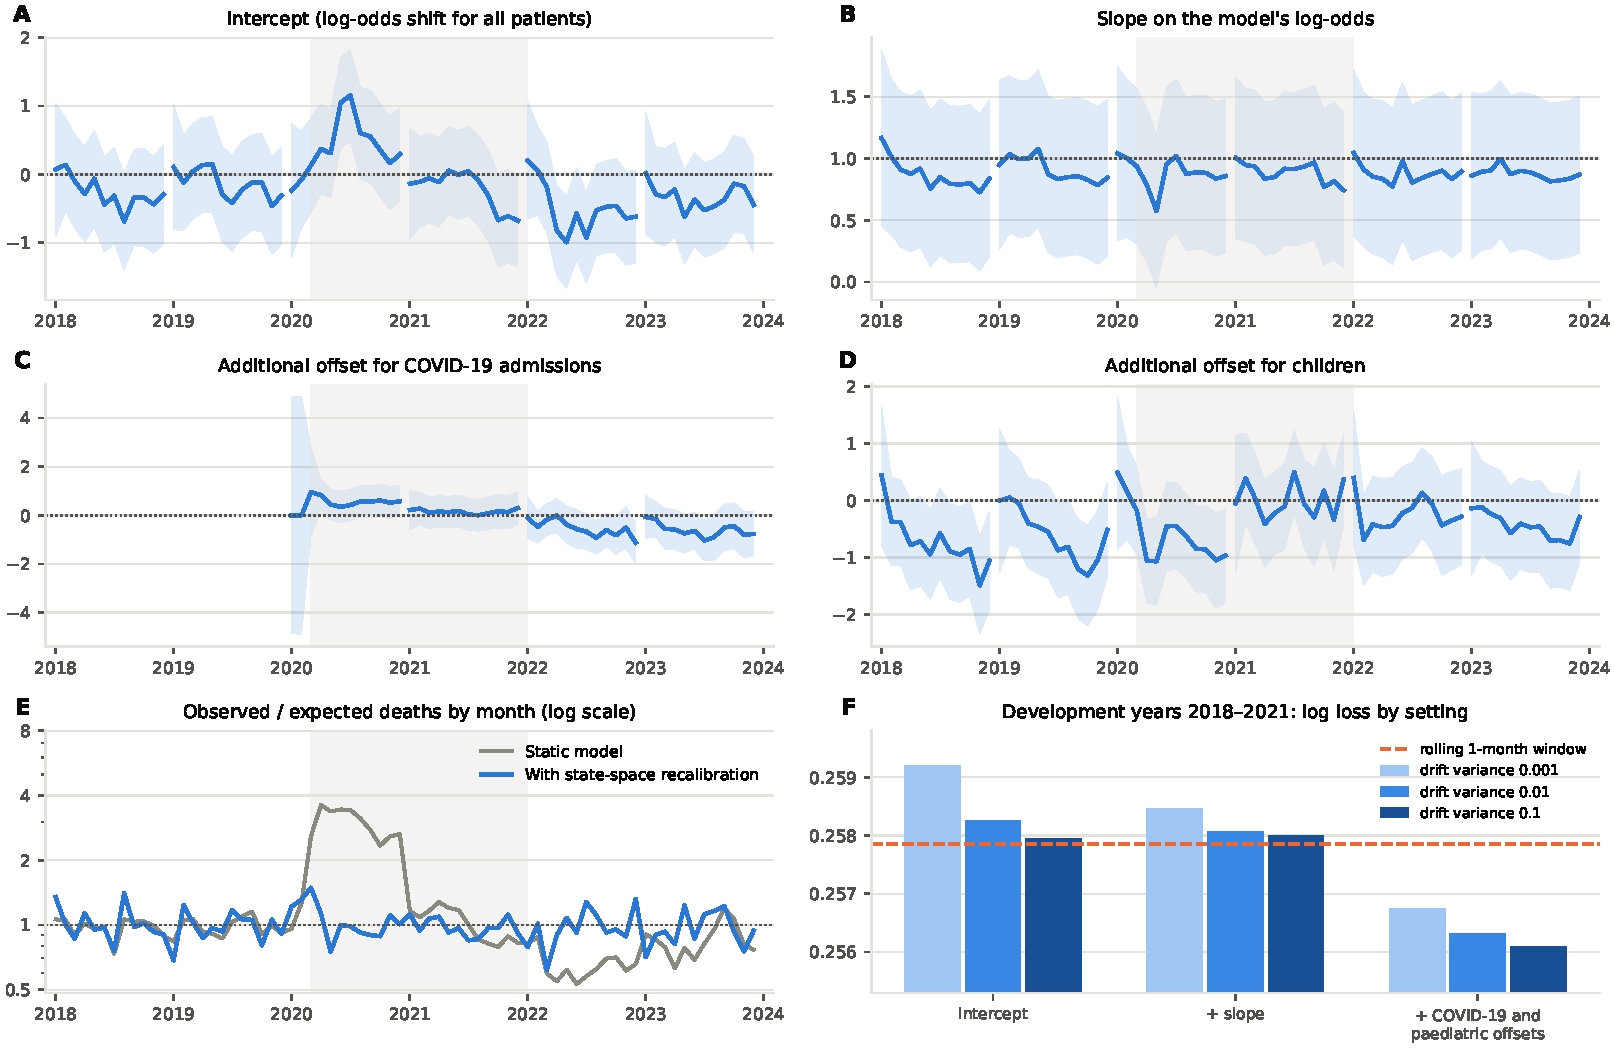
\includegraphics[width=\linewidth,height=92.655mm,keepaspectratio]{figures/x09_state_trajectory.pdf}
\captionof{figure}{State trajectories and O/E in annual forward evaluations from 2018 to 2023. Each year uses all preceding data for fitting, unlike the fixed development period in Figure 11.}\label{fig:traj}
\end{center}
In forward evaluation, the COVID-19 offset changed from approximately +0.49 in 2020 to $-$0.53 in 2022 and $-$0.60 in 2023 (Figure 12). The same score required corrections in opposite directions across periods, making a single fixed intercept unlikely to remain adequate. These changes support population-specific update terms, although their causes may include changes in severity, admission practice, treatment and coding.

\clearpage
\subheading{4.6 Ranking transfers to unseen provinces, but absolute probabilities still require adjustment}

\begin{center}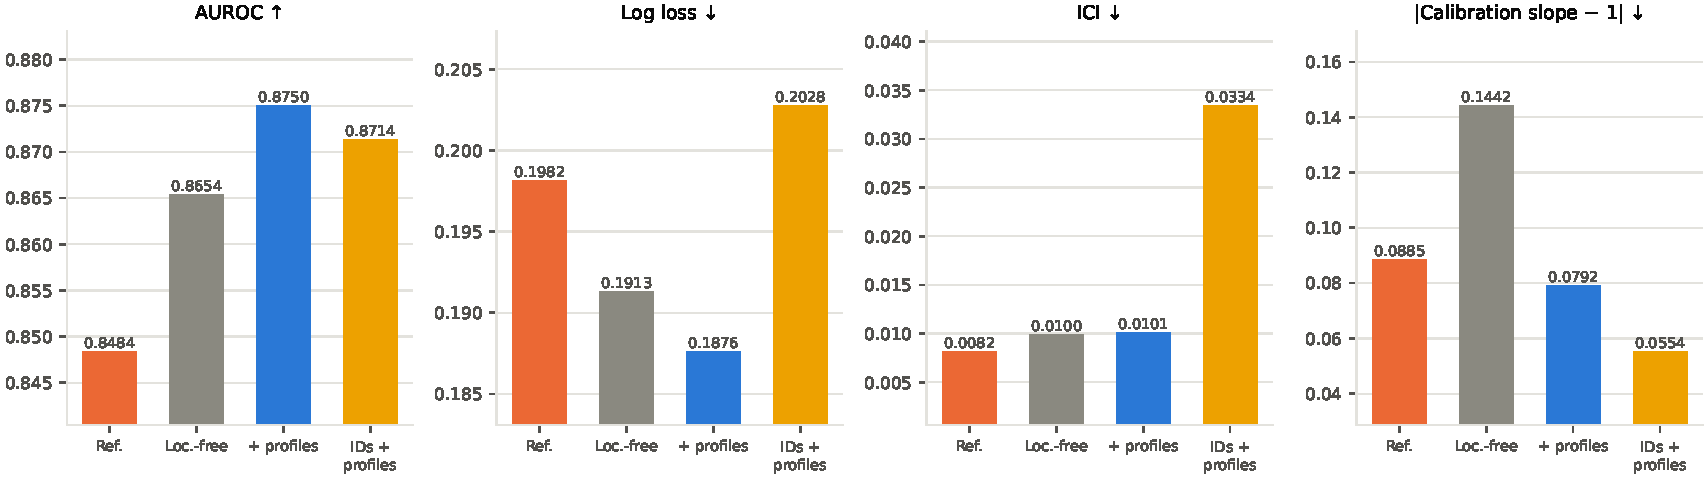
\includegraphics[width=\linewidth,height=90.795mm,keepaspectratio]{figures/t4_geographic_profiles.pdf}
\captionof{figure}{Configuration comparisons in province-held-out evaluation. The geographic profile configuration did not use the full HiCARE second layer, and configurations with and without profiles also differed in ensemble membership.}\label{fig:geoprof}
\end{center}
After removing geographic identifiers, the profile configuration increased AUROC from 0.8654 to 0.8750 and reduced log loss from 0.1913 to 0.1876 (Figure 13). However, the calibration intercept shifted from $-$0.004 to +0.171 and ICI from 0.0100 to 0.0101. Relative risk identification improved while overall risk remained underestimated. Because ensemble membership also changed, these differences support the transfer performance of the configuration as a whole and cannot be attributed exclusively to profiles.


\begin{center}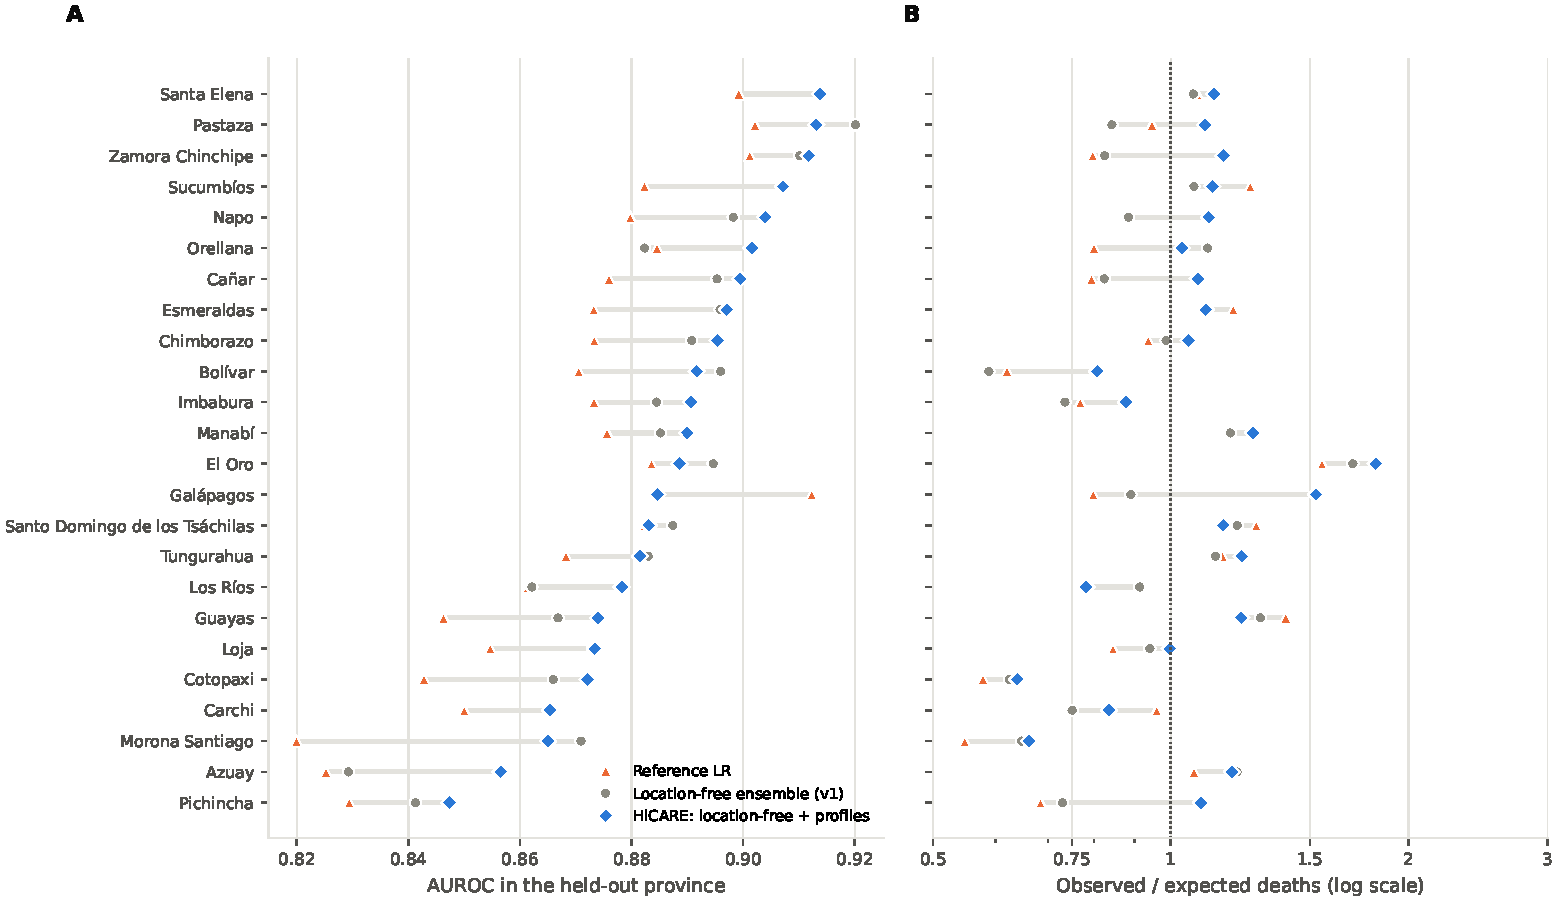
\includegraphics[width=\linewidth,height=90.795mm,keepaspectratio]{figures/x11_geo_by_province.pdf}
\captionof{figure}{AUROC and O/E within held-out provinces. The legacy HiCARE label denotes the geographic profile configuration. Provinces were excluded from direct model fitting, but their historical statistics remained available.}\label{fig:geoprov}
\end{center}
The profile configuration exceeded LR-7 in AUROC in 23 of 24 provinces, while median provincial absolute log(O/E) decreased from 0.18 without profiles to 0.15 with profiles (Figure 14). Improvement in a typical province can coexist with a non-zero national calibration intercept because the summaries use different weights. Facility profiles offer a candidate transferable representation, but both local ranking and probability levels require assessment before use. Complete comparisons across populations and protocols are provided in Table S6 and Figure S2.

\clearpage
\mainheading{5 Population monitoring with distinct reference models}
\subheading{5.1 Case-mix adjustment changes priorities for regional investigation}
Facility information that helps predict risk should not automatically become an adjustment variable when comparing regional outcomes. We therefore used an independent case-mix model that retained provincial and facility differences, with empirical Bayes estimation to stabilise small-sample ratios. Adjusted mortality ratios across 24 provinces ranged from 0.61 to 1.56; 95\% intervals were above 1 in ten provinces and below 1 in nine (Table S7).


\begin{center}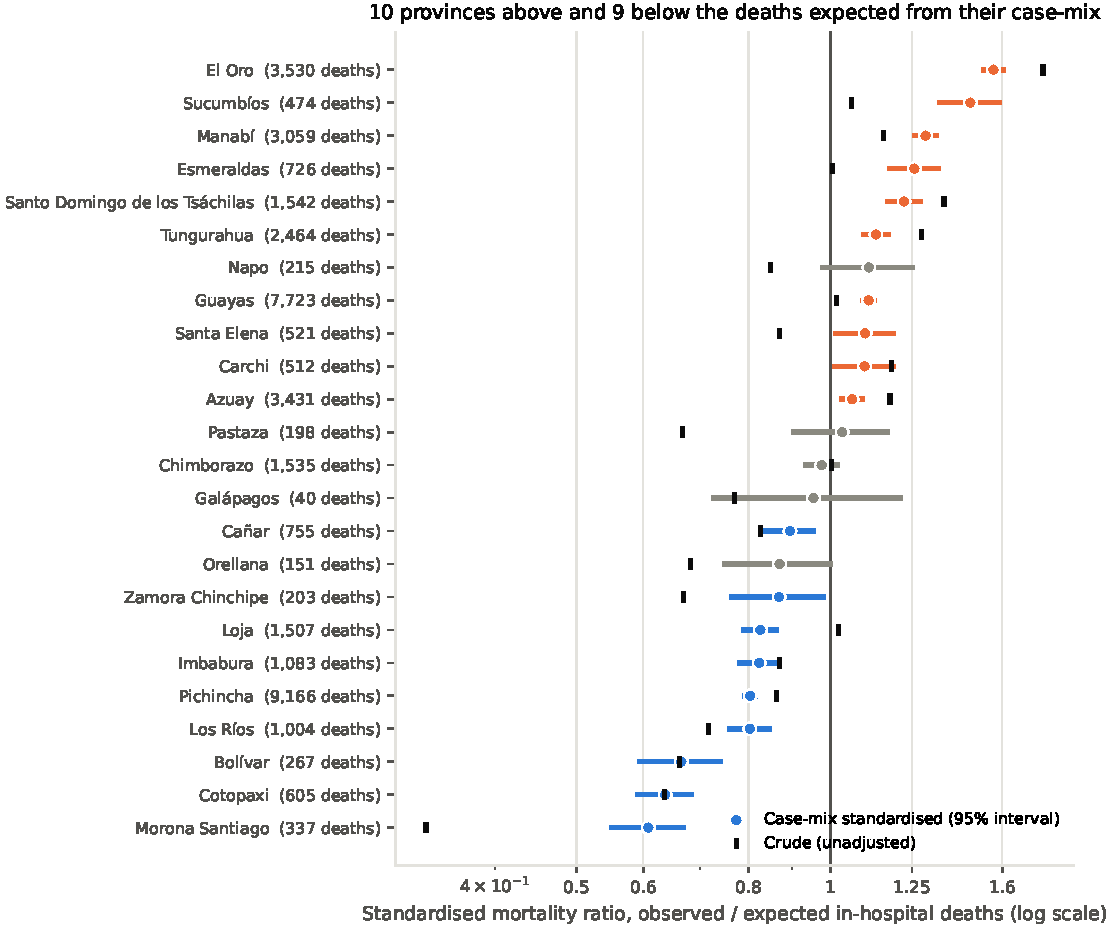
\includegraphics[width=\linewidth,height=190.59mm,keepaspectratio]{figures/m1_province_smr.pdf}
\captionof{figure}{Provincial case-mix-standardised in-hospital mortality ratios. Points and intervals show empirical Bayes estimates and 95\% intervals; vertical tick marks indicate crude ratios.}\label{fig:prov}
\end{center}
The crude ratio in Sucumbíos was 1.06, rising to 1.47 after adjustment (95\% interval 1.34–1.60). In Esmeraldas it increased from 1.01 to 1.26. Crude mortality close to the national average thus concealed higher mortality relative to the admitted case mix. In El Oro, adjustment reduced the ratio from 1.79 to 1.56 (1.51–1.61), suggesting that higher-risk admissions explained part, but not all, of the departure (Figure 15).

Adjustments in opposite directions show how crude mortality can both conceal and exaggerate regional differences. Standardisation helps identify where investigation should be directed; it does not establish that residual differences reflect quality of care. Without physiological severity measures and complete referral information, high adjusted values still require review of clinical records and registry data.

\clearpage
\subheading{5.2 Relative departures and death counts imply different review priorities}
The same relative departure can involve very different numbers of deaths. Provincial comparisons therefore retain both O/E and O$-$E. The ratio measures departure relative to case mix, whereas the difference measures its absolute scale. Figure 16 shows that the two summaries produce different priority rankings.


\begin{center}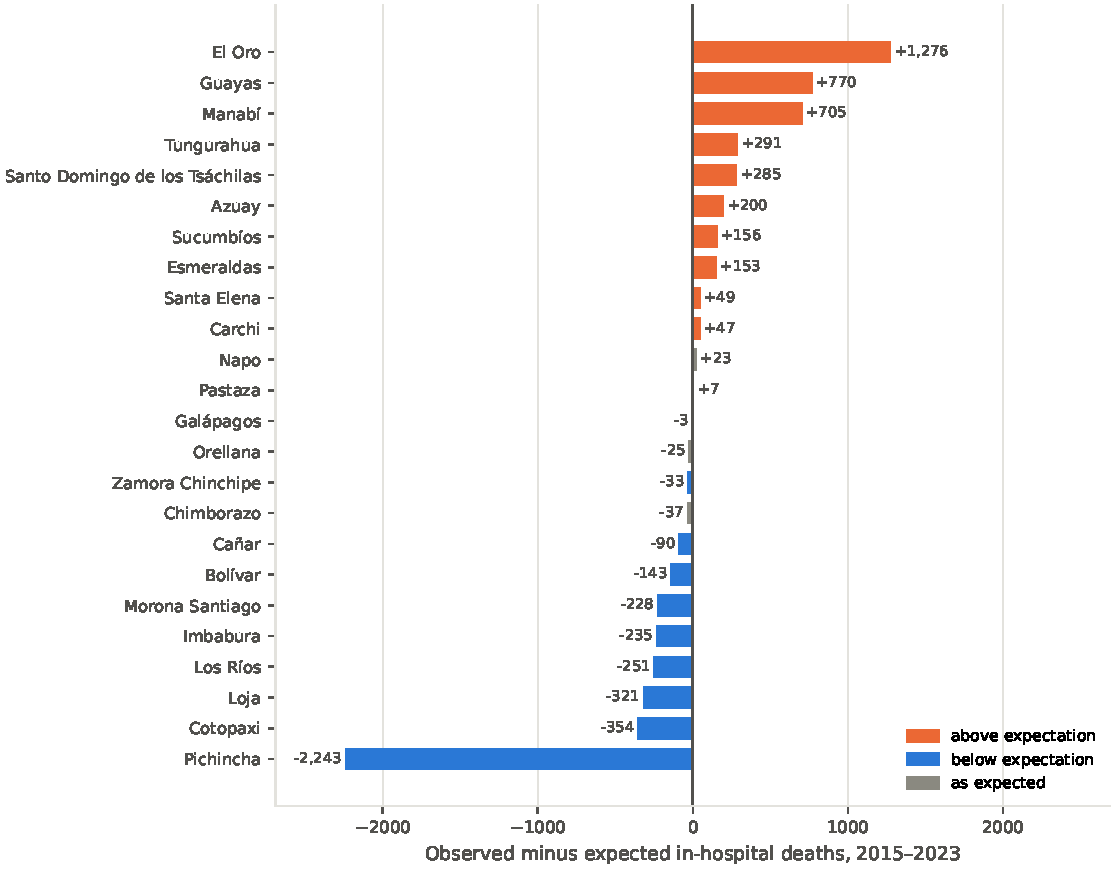
\includegraphics[width=\linewidth,height=194.155mm,keepaspectratio]{figures/x13_excess_deaths.pdf}
\captionof{figure}{Observed minus expected in-hospital deaths by province, 2015–2023.}\label{fig:excess}
\end{center}
Sucumbíos had a mortality ratio of 1.47 and approximately 156 more observed than expected deaths. Guayas had a smaller ratio of 1.11 but a difference of approximately 770 deaths, nearly five times as large. El Oro and Manabí combined substantial relative departures with differences of approximately 1,276 and 705 deaths, respectively. Reliance on ratios alone could overlook modest departures involving many admissions in populous regions.

The approximately 3,932 excess observed deaths across high-ratio provinces are a descriptive difference from the specified model reference. They include unmeasured severity, admission selection and registry differences and cannot be interpreted as avoidable deaths. Their immediate role is to indicate the scale of records requiring further investigation, alongside the strength of the relative departure. Additional results for facility groups and administering entities appear in Tables S8–S9 and Figures S3–S4.

\clearpage
\subheading{5.3 Overall departures must be located in time and population}

\begin{center}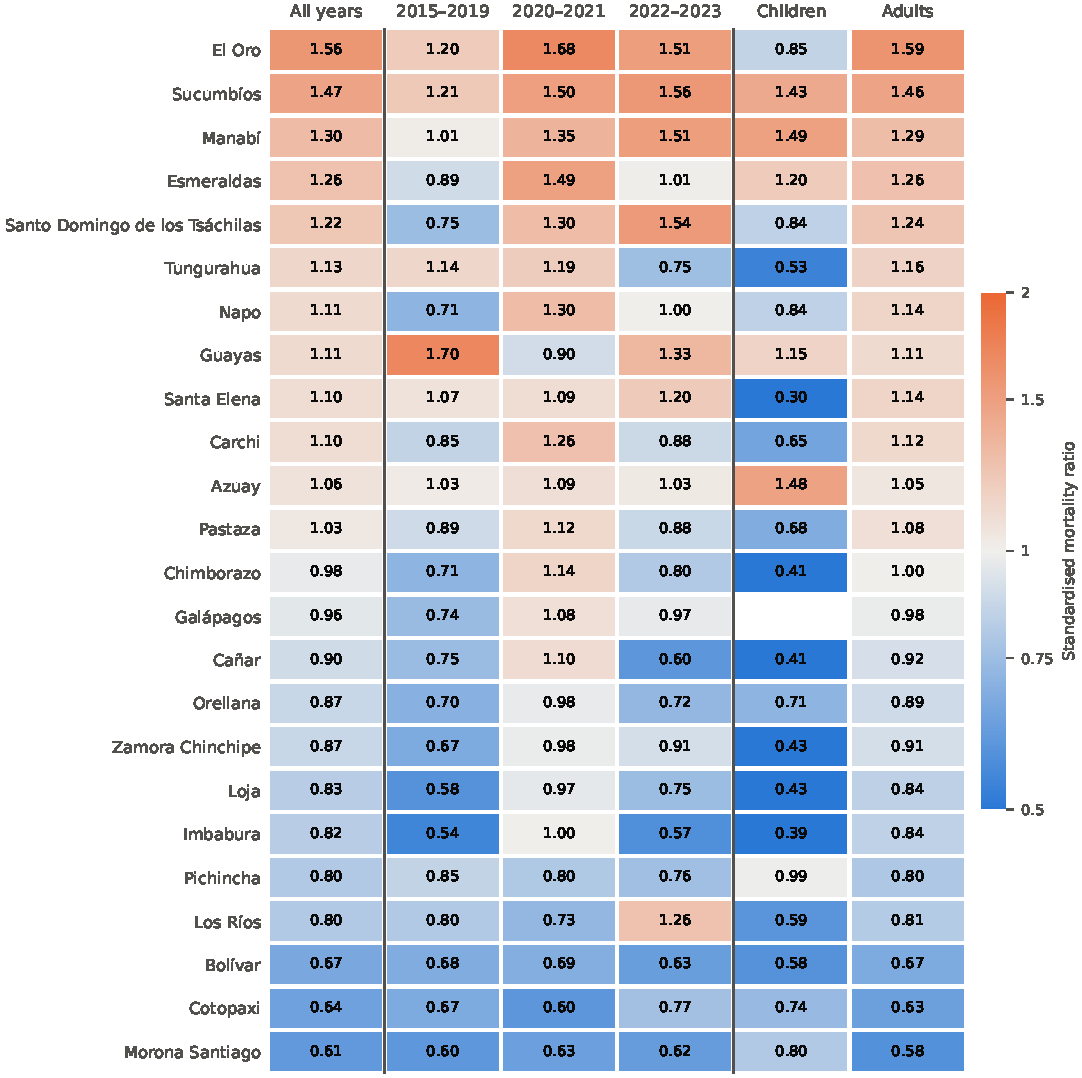
\includegraphics[width=\linewidth,height=195mm,keepaspectratio]{figures/x12_province_tilemap.pdf}
\captionof{figure}{Standardised mortality ratios by province, period and age stratum.}\label{fig:tilemap}
\end{center}
Period-specific estimates distinguished persistent departures from temporary changes. El Oro had mortality ratios of 1.20, 1.68 and 1.51 across the three periods, remaining high after the pandemic. Esmeraldas increased from 0.89 to 1.49 before returning to 1.01 (Figure 17). Investigation in El Oro should therefore consider longstanding admission and service characteristics, whereas the Esmeraldas pattern directs attention to changes during the early pandemic.

Age stratification further narrowed the population requiring investigation. El Oro had an adult mortality ratio of 1.59 and a paediatric ratio of 0.85, whereas Sucumbíos had ratios of 1.46 and 1.43, respectively. Both provinces had high overall ratios, but the affected populations differed. Combining relative ratios, absolute differences and stratified trajectories locates regional signals in particular periods and patient groups, beyond a national ranking.

\clearpage
\subheading{5.4 A fixed historical reference preserves period-specific departures in non-COVID outcomes}
Updating current probabilities absorbs recent changes in outcomes. Historical comparisons therefore used a separate clinical model trained in 2015–2019 and then held fixed. In 2020–2021, non-COVID ARI accounted for 3,485 observed deaths against 2,108 expected deaths, giving an O/E of 1.65 (95\% interval 1.60–1.71). The ratio returned to 0.97 in 2022–2023 (Table S10). This design preserved the early-pandemic departure and subsequent decline rather than gradually incorporating them into an updated baseline.


\begin{center}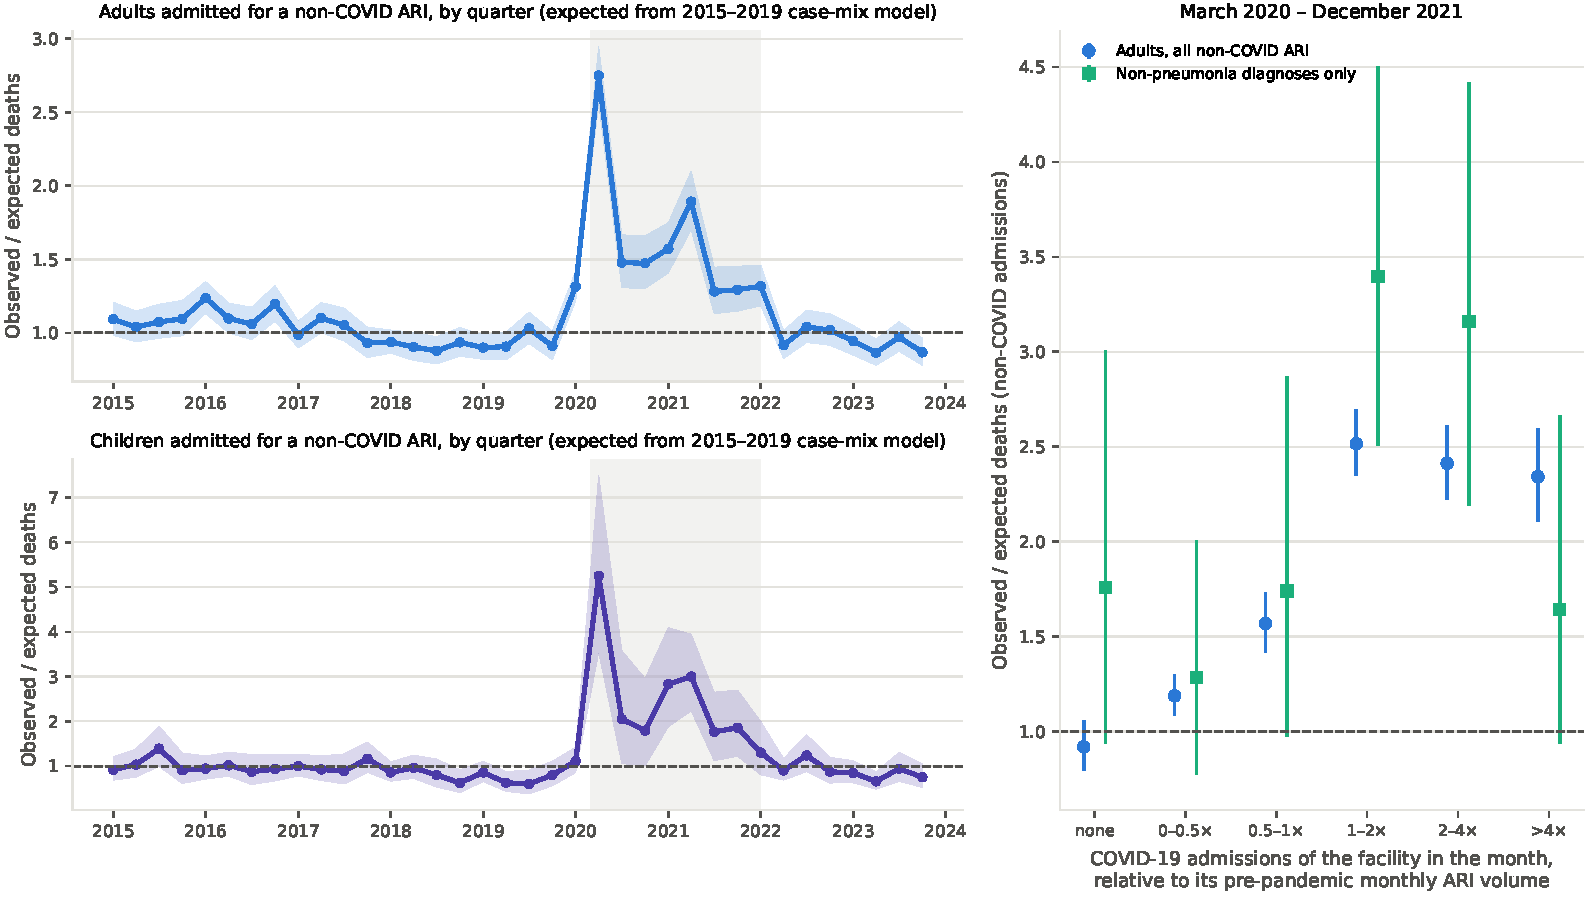
\includegraphics[width=\linewidth,height=187.95499999999998mm,keepaspectratio]{figures/m4_pandemic_strain.pdf}
\captionof{figure}{Quarterly non-COVID ARI mortality O/E (left) and stratification by facility COVID-19 demand (right). Shading denotes March 2020 to December 2021.}\label{fig:strain}
\end{center}
Departures were greater in facility-months with higher COVID-19 admission demand. Adult O/E was 0.92 without COVID-19 demand, rose to 2.52 when demand was one to two times historical mean monthly ARI admissions, and was 2.41 and 2.34 in the two higher categories (Table S11; Figure 18). The association plateaued at high demand rather than showing a continuously increasing dose–response. This demand ratio measures admissions relative to a historical benchmark, not bed occupancy or a capacity threshold.

This co-occurrence makes facility-months a useful scale for examining referral and admission processes. However, cumulative provincial demand and mortality ratios were not positively correlated (r = $-$0.19, p = 0.37; Figure S5). A contemporaneous facility-level association should therefore not be extrapolated to a province-wide effect. The sources of mortality departures require investigation at the corresponding spatial and temporal scale.

\clearpage
\subheading{5.5 Falling admissions can coexist with rising mortality risk among admitted patients}

\begin{center}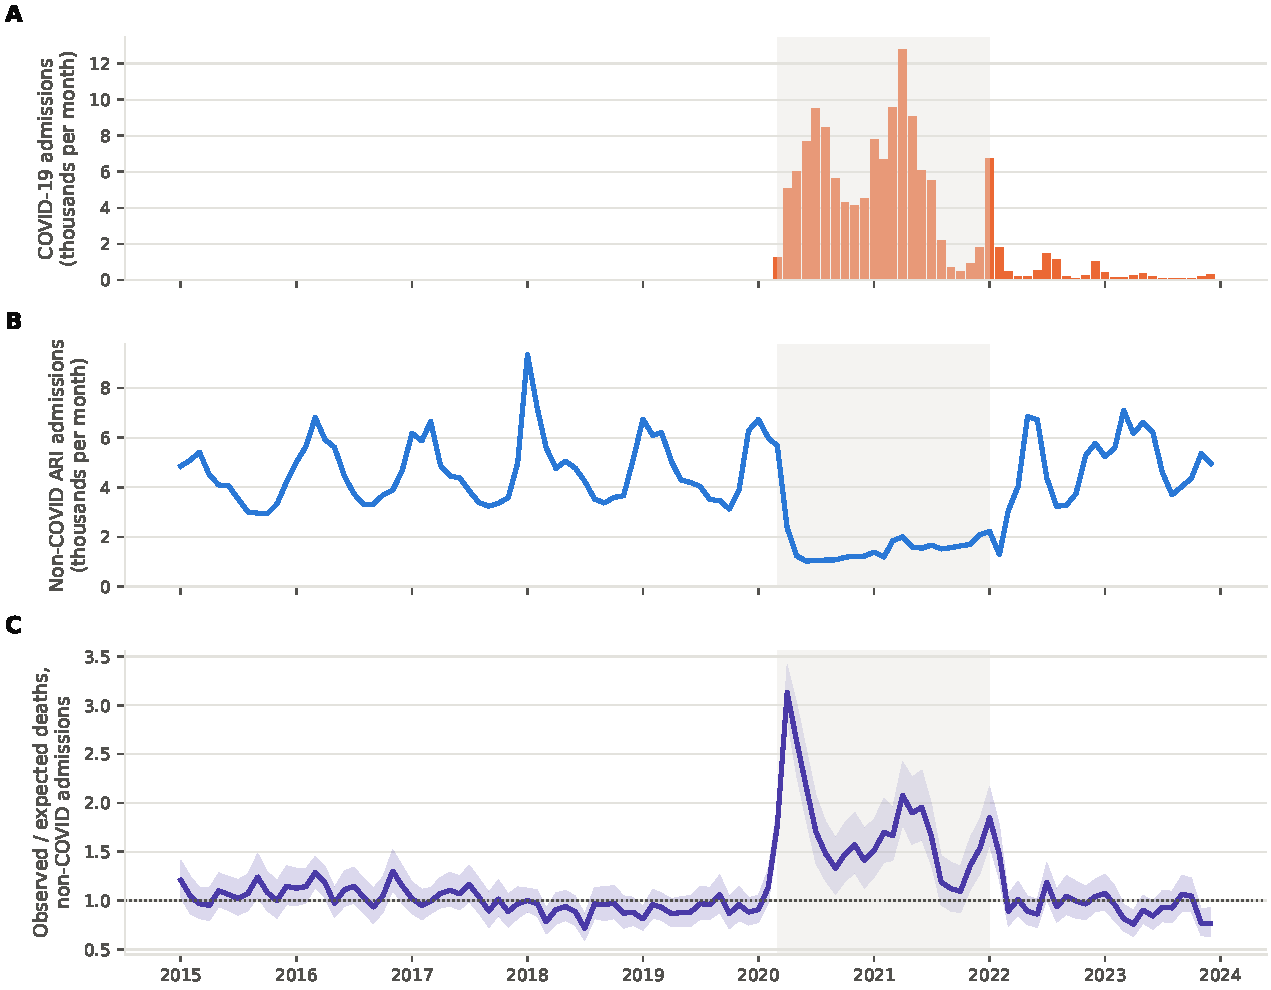
\includegraphics[width=\linewidth,height=194.62mm,keepaspectratio]{figures/x14_strain_timeline.pdf}
\captionof{figure}{Monthly (A) COVID-19 admissions, (B) non-COVID ARI admissions and (C) observed-to-expected mortality among non-COVID admissions.}\label{fig:timeline}
\end{center}
Non-COVID admissions declined during the pandemic while standardised mortality among admitted patients increased (Figure 19). Admission counts alone therefore did not capture changes in outcome burden. Reduced attendance by patients with mild illness, altered admission thresholds or concentrated referrals could leave fewer registered patients with greater risk. Case-mix adjustment accounted for some recorded differences, but remaining departures may still include incompletely recorded severity.

These findings are compatible with the dynamic calibration results. The dynamic model adapts to mortality probabilities in current patients, whereas the fixed historical model preserves changes relative to the past. Retaining both outputs could maintain usable current probabilities while identifying periods that warrant retrospective investigation. Good calibration after updating should not be mistaken for an unchanged service environment.

The study did not link patients treated outside hospital or those unable to obtain admission. These findings therefore concern admitted patients. Additional data are needed to assess disease burden and barriers to care outside the registry, limiting any inference that declining admissions imply declining population demand.

\clearpage
\subheading{5.6 Paediatric disparities direct attention to severity at arrival and pathways to care}
Sequential adjustment provided another perspective on population differences. Among adults, the Indigenous-to-Mestizo mortality ratio increased from 0.60 before adjustment to 0.78 after clinical adjustment and 1.01 after adding facility information. Among children, adjusted ratios remained 1.25 for rural residence (95\% interval 1.10–1.42) and 1.32 for Indigenous ethnicity (1.05–1.56). The ratio for children receiving care outside their canton of residence decreased from 3.99 to 2.55 (Table S12). The same adjustment thus had different implications across age groups, which an all-age summary would obscure.


\begin{center}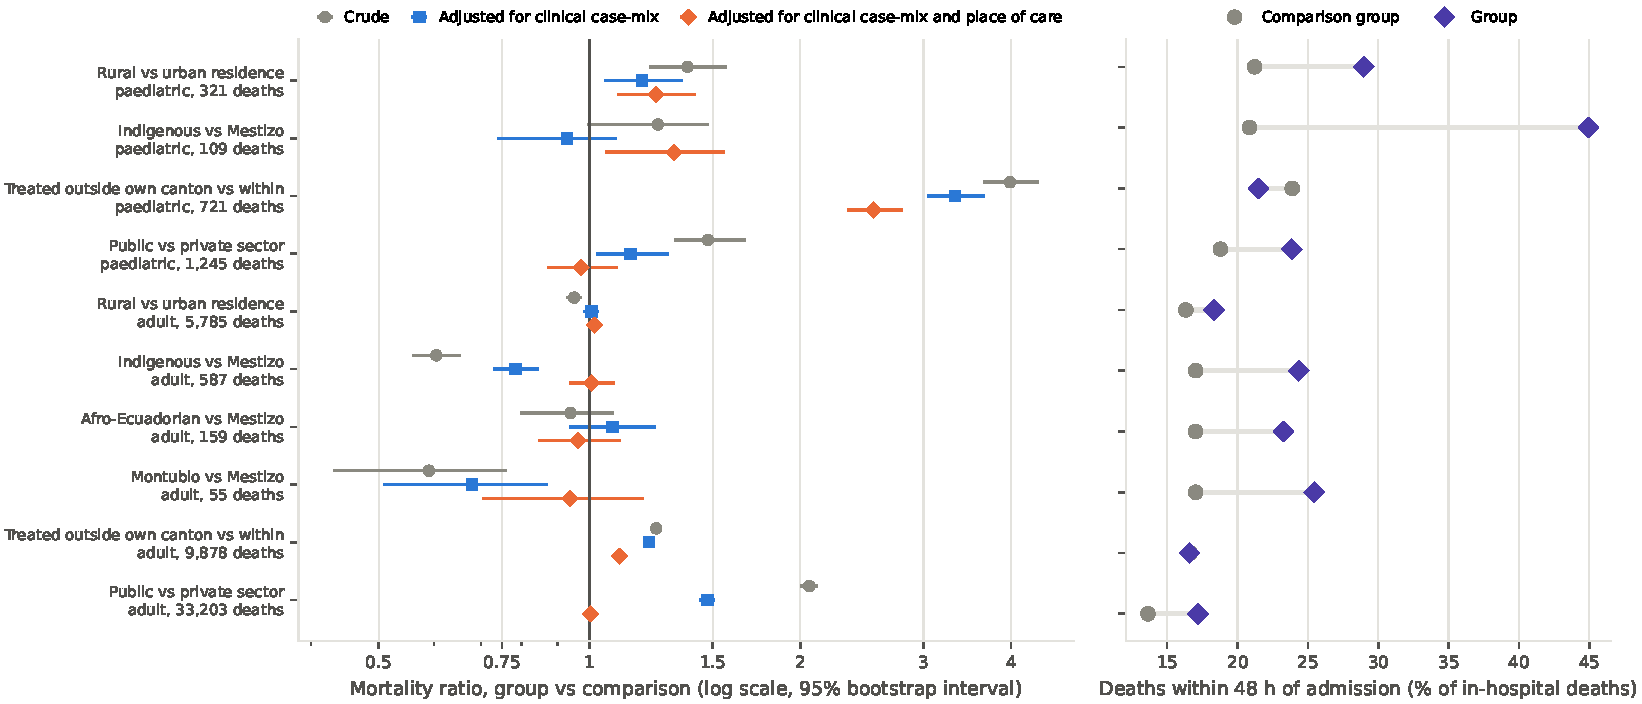
\includegraphics[width=\linewidth,height=186.56mm,keepaspectratio]{figures/m5_inequity.pdf}
\captionof{figure}{Sequentially adjusted relative mortality ratios across demographic groups (left) and the proportion of deaths occurring within 48 hours of admission (right).}\label{fig:ineq}
\end{center}
The timing of death further specified the paediatric disparity. Among children who died, approximately 45\% of Indigenous children died within 48 hours, compared with 21\% of Mestizo children. Corresponding proportions were approximately 29\% for rural and 21\% for urban children (Figure 20). The combination of higher adjusted mortality and a greater concentration of early deaths identifies severity at arrival, pre-hospital illness and referral pathways as priorities for further review.

These proportions use deaths as the denominator and do not represent early mortality risk among all children. Sequential adjustment describes associations under different conditioning sets; it does not establish causal mediation between ethnicity, facility selection and outcomes. Its role is to narrow the records and information requiring further investigation, rather than to identify a population attribute as a cause of death.

\clearpage
\subheading{5.7 Recovery in paediatric demand was concentrated at ages 1–9 years}
Paediatric admissions and deaths did not recover in parallel. Relative to the fixed pre-pandemic seasonal benchmark, non-COVID admissions in 2023 were 1.32 times expected (95\% prediction interval 1.23–1.43), whereas deaths were 1.00 times expected (0.84–1.19). Including a long-term trend reduced the admission ratio to 1.11 (0.97–1.27), showing that the estimated rebound depended on assumptions about historical trends (Table S13). This sensitivity affects the strength of the evidence for demand exceeding historical expectations, but not the clear recovery from the early-pandemic trough.


\begin{center}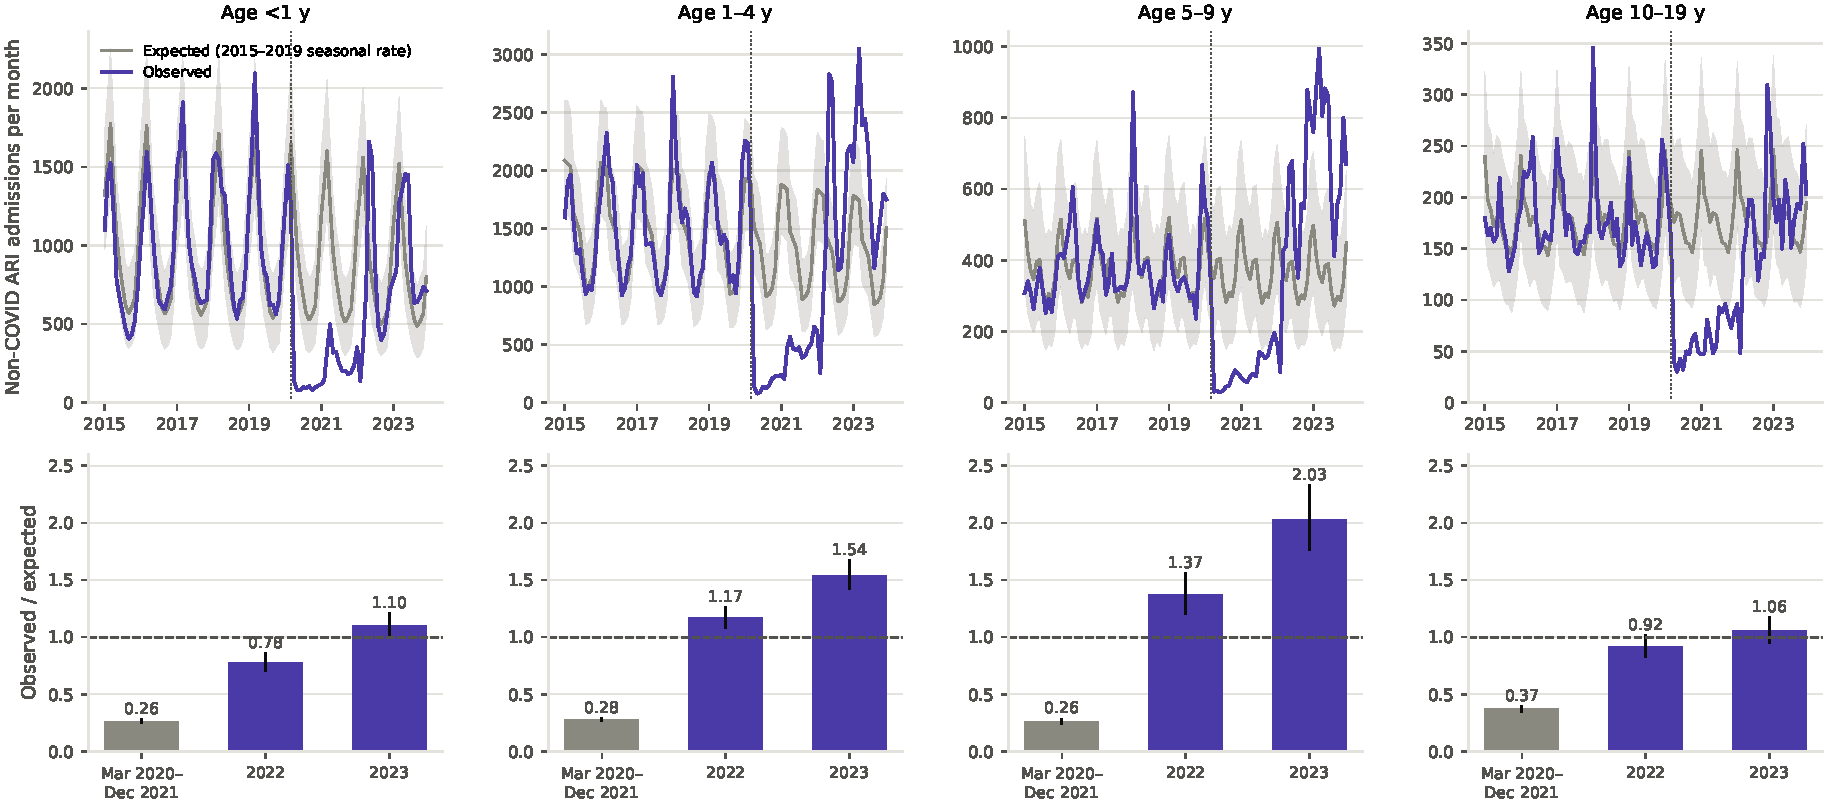
\includegraphics[width=\linewidth,height=90.2525mm,keepaspectratio]{figures/m6_paediatric_rebound.pdf}
\captionof{figure}{Paediatric non-COVID ARI admissions by age group compared with a pre-pandemic seasonal counterfactual.}\label{fig:rebound}
\end{center}
Age-specific estimates showed admission ratios of 1.54 at ages 1–4 and 2.03 at ages 5–9 in 2023, compared with 1.10 in infants and 1.06 at ages 10–19 (Figure 21). The increase was concentrated in older children; the annual aggregate did not imply proportional increases in every age group.


\begin{center}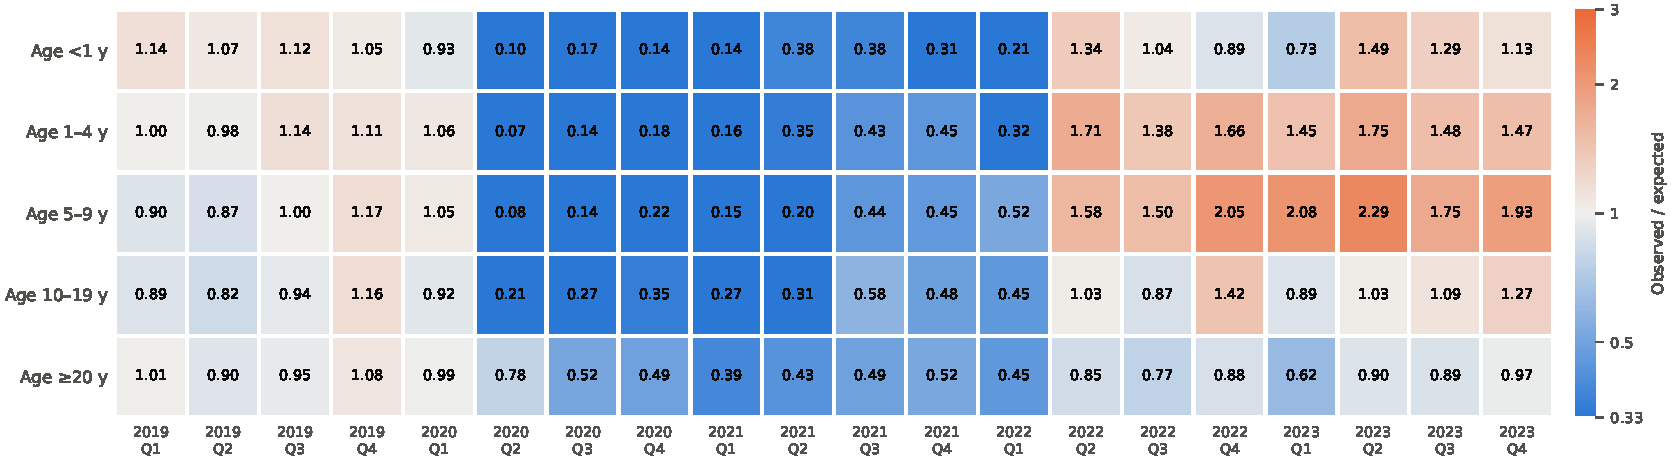
\includegraphics[width=\linewidth,height=90.2525mm,keepaspectratio]{figures/x16_rebound_tilemap.pdf}
\captionof{figure}{Observed-to-expected non-COVID ARI admission ratios by age group and quarter, 2019–2023.}\label{fig:rebtile}
\end{center}
Quarterly estimates located the recovery more precisely. All paediatric groups remained below baseline in the first quarter of 2022, but ratios rose to 1.71 at ages 1–4 and 1.58 at ages 5–9 in the second quarter. The latter group reached 2.29 in the second quarter of 2023 (Figure 22). This concentration by age and time supports stratified monitoring of admission demand.

\clearpage
\subheading{5.8 Age shifts accompanied changes in syndrome mix and seasonality}

\begin{center}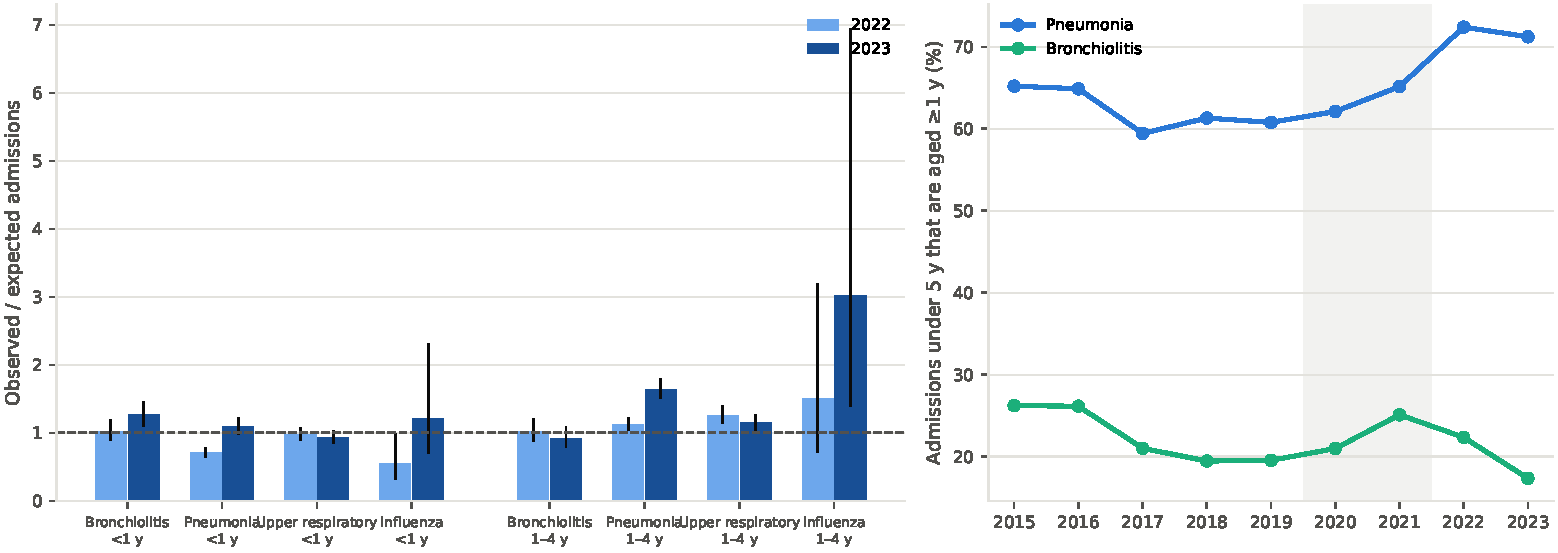
\includegraphics[width=\linewidth,height=90.95mm,keepaspectratio]{figures/m7_syndromes_age_shift.pdf}
\captionof{figure}{Syndrome-specific admissions and age composition in children under 5 years. The right-hand panel shows the proportion aged 1–4 among under-5 admissions for each syndrome.}\label{fig:syndromes}
\end{center}
The increase in older children was associated with pneumonia admissions. In 2023, pneumonia admissions at ages 1–4 were approximately 1.64 times the fixed benchmark. Among pneumonia admissions in children under 5, the proportion aged at least 1 year increased from approximately 62\% to 72\% (Figure 23). Recovery in paediatric demand therefore changed both admission volume and the age composition of patients requiring care.


\begin{center}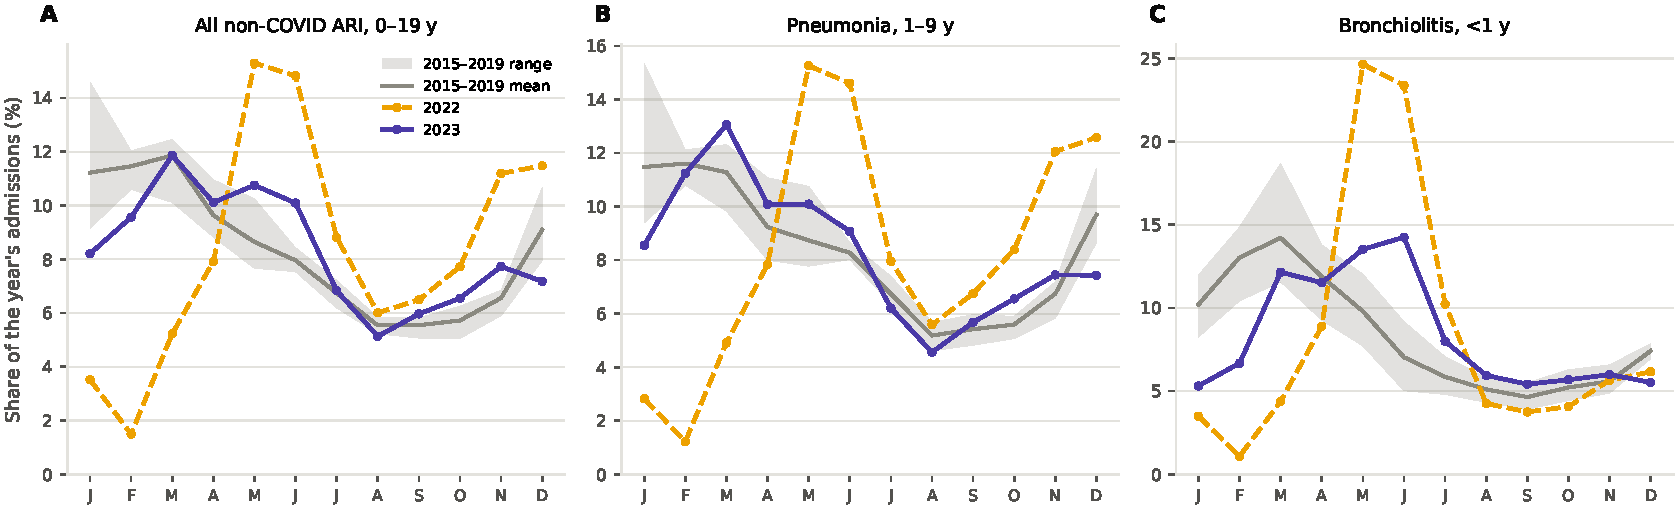
\includegraphics[width=\linewidth,height=90.95mm,keepaspectratio]{figures/x17_seasonality.pdf}
\captionof{figure}{Within-year monthly distributions of paediatric admissions before the pandemic and in 2022 and 2023.}\label{fig:season}
\end{center}
Seasonal recovery also differed by syndrome. Before the pandemic, pneumonia at ages 1–9 peaked mainly in January–February, whereas infant bronchiolitis peaked in February–March. Both shifted to May–June in 2022. In 2023, correlations with the pre-pandemic monthly distribution were 0.83 for pneumonia and 0.44 for bronchiolitis (Figure 24). An aggregated curve could conceal these differences, supporting separate local monitoring of pneumonia in older children and bronchiolitis in infants.

Together with evidence of seasonal heterogeneity in Ecuador [20], these observations support population- and syndrome-specific monitoring windows. Diagnostic codes and approximate population denominators remain insufficient to identify immune mechanisms or directly determine the optimal timing of preventive measures.

\clearpage
\subheading{5.9 National growth in demand does not determine local volume}

\begin{center}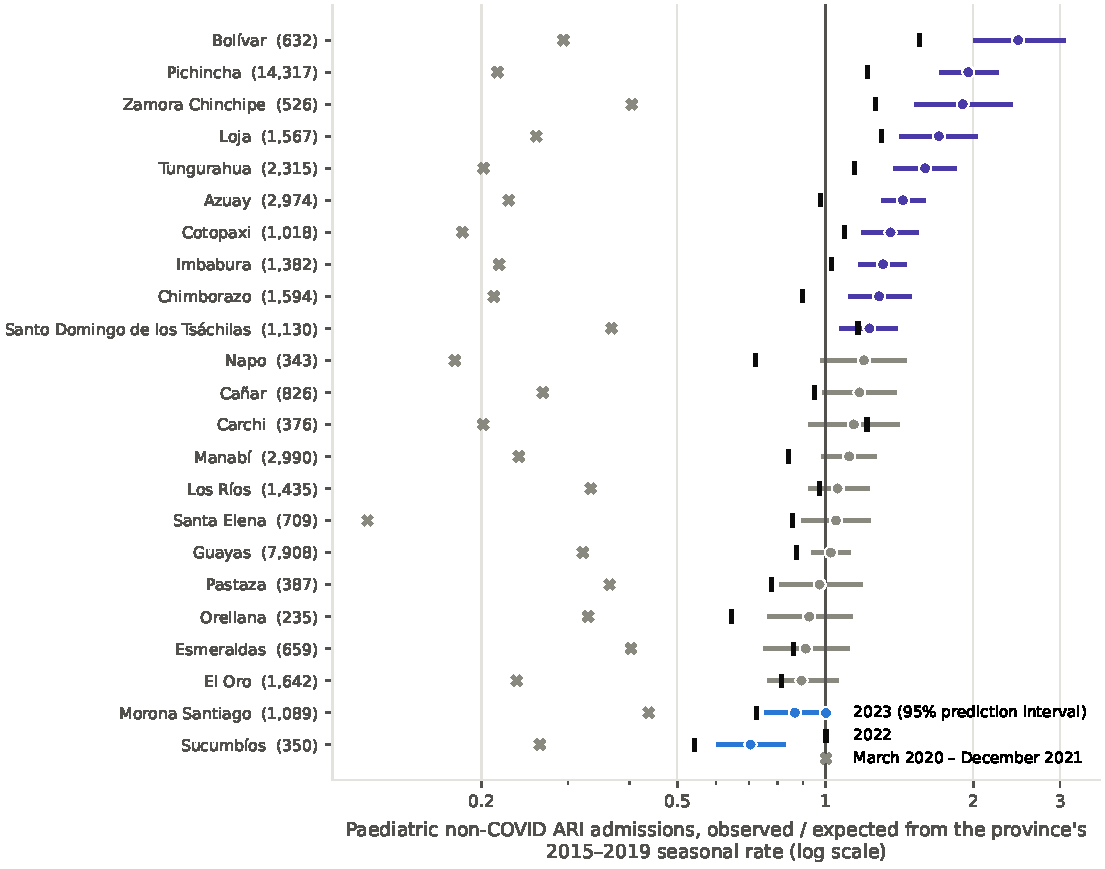
\includegraphics[width=\linewidth,height=194.0mm,keepaspectratio]{figures/x20_rebound_by_province.pdf}
\captionof{figure}{Paediatric non-COVID ARI admissions in 2023 relative to each province’s own pre-pandemic seasonal incidence.}\label{fig:rebprov}
\end{center}
In 2023, paediatric non-COVID admissions exceeded the provincial seasonal reference in ten provinces and fell below it in two. Ratios were 2.47 in Bolívar, 1.95 in Pichincha, 1.90 in Zamora Chinchipe and 1.70 in Loja, compared with approximately 1.03 in Guayas (Figure 25). The national estimate combined regions with markedly different growth and could not provide a uniform proportion for local paediatric preparedness.

Pichincha combined a high ratio with a large admission volume, whereas Bolívar had a larger relative increase from a smaller baseline. The former suggests a substantial absolute increase in admissions; the latter indicates a pronounced departure from the local historical pattern. As with reporting O/E alongside O$-$E in mortality monitoring, demand monitoring requires both relative changes and actual counts.

These results provide testable strata for subsequent service planning. Linking length of stay, bed turnover and staffing would be necessary to estimate how changes in admissions translate into capacity shortfalls. The present analysis identifies regions, populations and months requiring attention; it does not estimate the number of additional beds or staff needed.

\clearpage
\subheading{5.10 Risk stratification supports review priorities, while probability scales require maintenance}

\begin{center}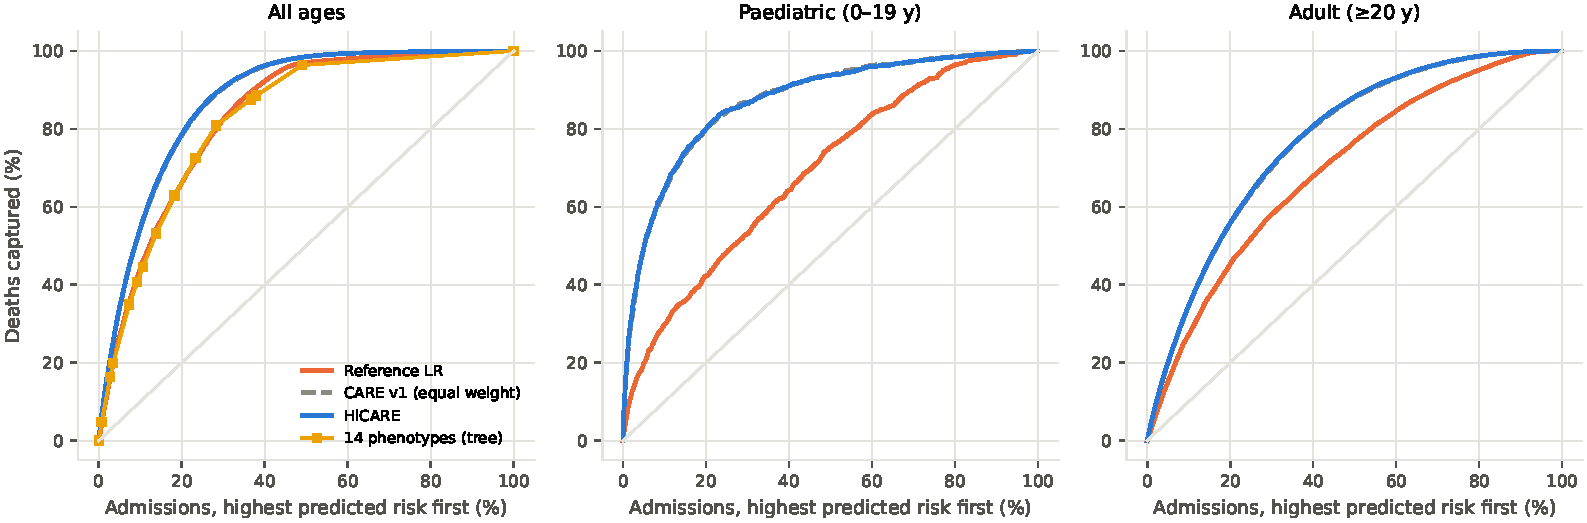
\includegraphics[width=\linewidth,height=92.4225mm,keepaspectratio]{figures/x18_concentration.pdf}
\captionof{figure}{Proportion of deaths captured when prioritising a given proportion of admission records. The 14-phenotype curve is used only for the all-age comparison.}\label{fig:conc}
\end{center}
HiCARE and EW had similar mortality-coverage curves, both more concentrated than LR-7. All-age continuous scores also outperformed ranking by 14 phenotypes (Figure 26). The seven highest-risk shallow-tree phenotypes comprised approximately 14\% of admissions and 53\% of deaths (Table S14; Figure S6), providing readable patient groupings. Continuous scores further differentiated priorities within those groups. The two representations therefore serve interpretation and ranking, respectively.


\begin{center}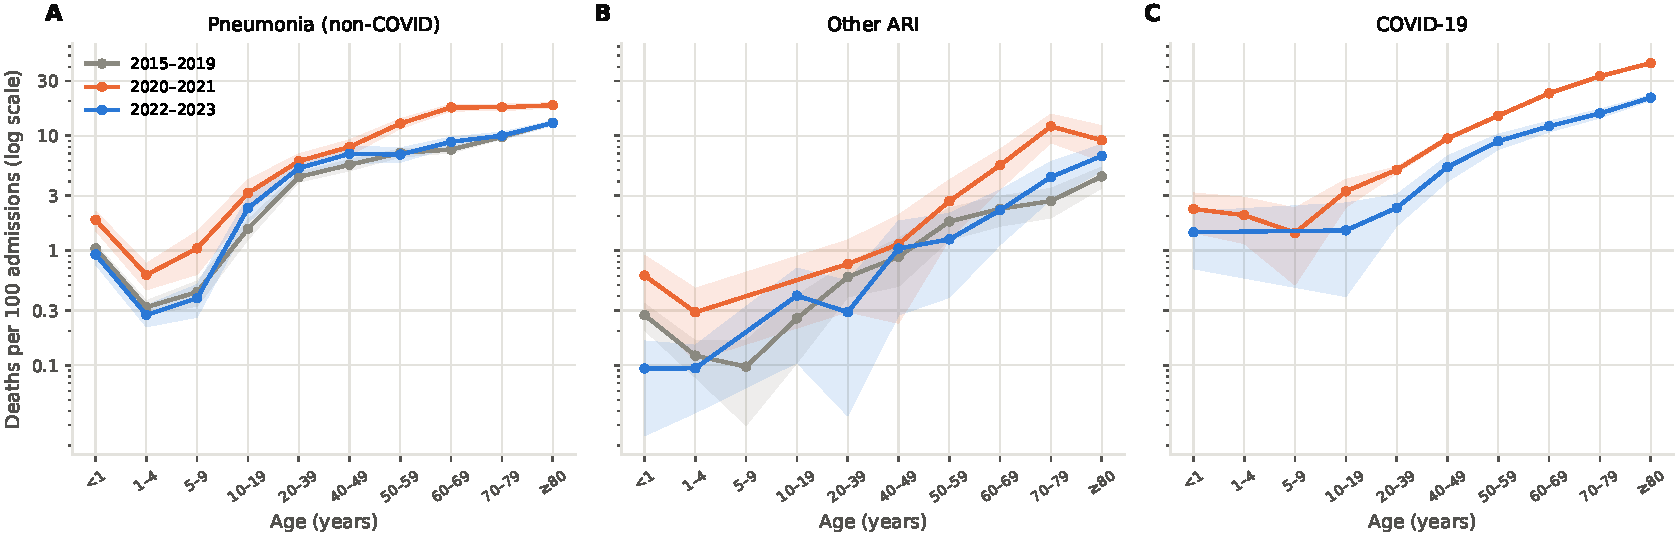
\includegraphics[width=\linewidth,height=92.4225mm,keepaspectratio]{figures/x19_age_mortality.pdf}
\captionof{figure}{Observed deaths per 100 admissions by age, infection group and period, with 95\% interval bands.}\label{fig:agemort}
\end{center}
Mortality at the same age also varied by infection type and period. Adult non-COVID pneumonia mortality was higher in 2020–2021, whereas COVID-19 mortality declined in 2022–2023 (Figure 27), consistent with the changing offsets in temporal calibration. Fixed phenotypes help explain where risk is concentrated, but their associated probabilities require maintenance over time.

Retrospective review could therefore retain interpretable grouping rules, continuous within-group rankings and current probabilities. This combination describes a potential workflow. Whether it reduces review costs or improves outcomes requires prospective evaluation with explicit action rules.

\clearpage
\mainheading{6 Discussion}
\subheading{6.1 Reliable monitoring requires distinct forms of evidence}
The principal finding is that strong risk ranking, reliable group-level probabilities and interpretable historical references must be established separately. The base ensemble supplied most discrimination, stratified calibration chiefly corrected predicted totals in specified populations, and monthly updating adapted the probability scale to later periods. Independent standardisation further showed that the effects of case mix, service context and temporal change on monitoring conclusions cannot be summarised by a single predictive metric.

This separation gives calibration gains a more specific interpretation. Expected deaths are sums of individual probabilities, so even modest systematic errors can accumulate into substantial differences in large populations. Marginal projection improved this aggregation property, but the small increase in worst-group ECE showed that group means cannot replace within-group accuracy. The findings connect with multicalibration research on population-specific errors [6,14], while remaining limited to the specified categories and evaluated held-out records.

EW approached HiCARE when given the same temporal update, and a single LightGBM retained most performance. These comparisons identify where gains arose. For registry monitoring, maintaining information quality, checking group errors and updating probabilities may matter more than increasing ensemble complexity. Implementation could begin with a simpler configuration and retain additional components only when they improve the errors relevant to the intended use.

\subheading{6.2 Facility profiles and fixed references serve different purposes}
Non-ARI profiles used routine records from other diseases at the same facility to describe the population served, supplementing ARI records with limited clinical detail. Attribution and province-held-out evaluation supported the use of this information, but did not separate case complexity, referral patterns and care quality. Profiles are therefore candidate risk representations rather than direct facility-quality scores. Estimating their independent contribution requires comparisons with identical ensemble members and strictly isolated historical information.

Whether information belongs in an expected value also depends on the comparison. For current patients, facility context may help estimate risk in the environment where care is received. For regional outcome investigation, controlling for the same context may absorb differences that require explanation. Temporal updating has the same property. Good calibration indicates adaptation to current mortality, not an unchanged historical risk relationship [7,17]. Retaining current probabilities alongside fixed historical references therefore separates prediction maintenance from outcome evaluation.

\subheading{6.3 From monitoring signals to further investigation}
Regional findings separated review priorities into the strength, scale and persistence of mortality departures. Paediatric findings showed that rising admissions could coincide with age shifts and altered seasonality without a proportional increase in deaths. Both support choosing the aggregation scale to match the question. High regional mortality requires additional information on severity and referral, whereas paediatric demand increases require linkage to length of stay and capacity. This study identifies populations and periods for those investigations without demonstrating improved outcomes following implementation.

\clearpage
\subheading{6.4 Scope of inference and next-stage validation}
Registry information limits the interpretation of outcome differences. The data lack complete comorbidity, physiological severity, laboratory, vaccination and patient-linkage information, and facility groups may combine multiple hospitals. Residual differences after standardisation can therefore arise from unmeasured severity, repeated admissions and admission selection. Observed-minus-expected deaths can guide record review but do not measure avoidable deaths; sequential adjustment does not constitute causal mediation analysis.

The validation protocols also constrain prospective and transfer claims. Discharge diagnoses were not confirmed to be available at admission; historical aggregates did not fully isolate earlier labels from held-out records or regions; and monthly updating did not simulate actual reporting delays. The provincial experiment changed both profiles and ensemble membership and did not run the full second layer. Subsequent validation should restrict predictors to those available at admission, reconstruct features within strictly rolling historical windows and compare identical learners across facilities to determine how much performance is retained.

Uncertainty estimates did not cover the entire analysis. The main experiments used a single training seed, paired resampling operated at the record level, and most intervals did not propagate model refitting or within-facility dependence. Global Platt calibration of out-of-fold standardisation probabilities used all outcomes. O/E intervals generally conditioned on fixed expected deaths, and regional screening did not adjust for multiple comparisons. Regional signals are therefore exploratory priorities for investigation rather than definitive rankings of facility performance.

Paediatric extrapolation was sensitive to long-term trend assumptions, and infants and children aged 1–4 shared the population trajectory for ages 0–4. These conditions limit interpretation of fine age-specific changes and departures from historical trends. Separate population series and later observations would help distinguish short-term recovery from sustained demand changes. Practical utility requires a separate evaluation with prespecified review proportions and action rules, recording findings, workload and outcomes to test whether retrospective concentration translates into service benefits.

\mainheading{7 Conclusion}
Historical facility profiles, stratified calibration and temporal updating served different roles in national admission data. Strong base models supplied most risk ranking, while group correction and continued maintenance improved probability estimates. Independent case-mix and historical references provided distinct scales for interpreting regional mortality and paediatric admission demand. Reporting these outputs separately yields concrete leads for record review and local service preparation. Prospective applicability and practical benefits still require validation with strict information timing and explicit action pathways.

\subheading{Data sources and study declarations}
The study used publicly available INEC hospital-bed and discharge registry data and historical annual releases [33]. This manuscript is a research revision. Manuscript sources, figures and accompanying analysis code are available at \url{https://github.com/liProj/hicare-ari-manuscript}. Detailed methods, complete numerical results and supplementary figures are provided in the Supplementary Appendix.

\clearpage
\mainheading{References}
{\small [1] Fitzpatrick T, Buchan SA, et al. Pediatric Acute Respiratory Virus Hospitalizations: A Population-Based Cohort Study, 2017-2024. The Journal of Infectious Diseases, 2025;232(1):e137-e149. \url{https://doi.org/10.1093/infdis/jiaf212}\par}
{\small [2] Winthrop ZA, Perez JM, Staffa SJ, McManus ML, Duvall MG. Pediatric Respiratory Syncytial Virus Hospitalizations and Respiratory Support After the COVID-19 Pandemic. JAMA Network Open, 2024;7(6):e2416852. \url{https://doi.org/10.1001/jamanetworkopen.2024.16852}\par}
{\small [3] Grinsztajn L, Oyallon E, Varoquaux G. Why do tree-based models still outperform deep learning on typical tabular data? Advances in Neural Information Processing Systems, 2022;35. \url{https://papers.nips.cc/paper_files/paper/2022/hash/0378c7692da36807bdec87ab043cdadc-Abstract.html}\par}
{\small [4] Gorishniy Y, Kotelnikov A, Babenko A. TabM: Advancing Tabular Deep Learning with Parameter-Efficient Ensembling. International Conference on Learning Representations, 2025. \url{https://openreview.net/forum?id=Sd4wYYOhmY}\par}
{\small [5] Hollmann N, Müller S, Purucker L, et al. Accurate predictions on small data with a tabular foundation model. Nature, 2025;637:319–326. \url{https://doi.org/10.1038/s41586-024-08328-6}\par}
{\small [6] La Cava WG, Lett E, Wan G. Fair admission risk prediction with proportional multicalibration. Proceedings of the Conference on Health, Inference, and Learning. PMLR, 2023;209:350-378. \url{https://proceedings.mlr.press/v209/la-cava23a.html}\par}
{\small [7] Levy TJ, Coppa K, Cang J, et al. Development and validation of self-monitoring auto-updating prognostic models of survival for hospitalized COVID-19 patients. Nature Communications, 2022;13:6812. \url{https://doi.org/10.1038/s41467-022-34646-2}\par}
{\small [8] Davis SE, Dorn C, Park DJ, Matheny ME. Emerging algorithmic bias: fairness drift as the next dimension of model maintenance and sustainability. Journal of the American Medical Informatics Association, 2025;32(5):845-854. \url{https://doi.org/10.1093/jamia/ocaf039}\par}
{\small [9] Scheid MR, Friedmann B, Oppenheim M, et al. Development and validation of a clinical wearable deep learning based continuous inhospital deterioration prediction model. Nature Communications, 2025;16:9513. \url{https://doi.org/10.1038/s41467-025-65219-8}\par}
{\small [10] Singh H, Mhasawade V, Chunara R. Generalizability challenges of mortality risk prediction models: A retrospective analysis on a multi-center database. PLOS Digital Health, 2022;1(4):e0000023. \url{https://doi.org/10.1371/journal.pdig.0000023}\par}
{\small [11] Yang J, Dung NT, Thach PN, et al. Generalizability assessment of AI models across hospitals in a low-middle and high income country. Nature Communications, 2024;15:8270. \url{https://doi.org/10.1038/s41467-024-52618-6}\par}
{\small [12] Duan M, Liu X, Yeung W, et al. Multicenter validation and updating of the ELDER-ICU model for severity assessment in elderly critical illness. npj Digital Medicine, 2026;9:498. \url{https://doi.org/10.1038/s41746-026-02472-1}\par}
{\small [13] Ktena I, Wiles O, Albuquerque I, et al. Generative models improve fairness of medical classifiers under distribution shifts. Nature Medicine, 2024;30:1166–1173. \url{https://doi.org/10.1038/s41591-024-02838-6}\par}
{\small [14] Globus-Harris I, Harrison D, Kearns M, Roth A, Sorrell J. Multicalibration as Boosting for Regression. Proceedings of the 40th International Conference on Machine Learning. PMLR, 2023;202:11459-11492. \url{https://proceedings.mlr.press/v202/globus-harris23a.html}\par}
{\small [15] Cabanillas Silva P, Sun H, Rezk M, et al. Longitudinal Model Shifts of Machine Learning–Based Clinical Risk Prediction Models: Evaluation Study of Multiple Use Cases Across Different Hospitals. Journal of Medical Internet Research, 2024;26:e51409. \url{https://doi.org/10.2196/51409}\par}
{\small [16] Kagerbauer SM, Ulm B, Podtschaske AH, et al. Susceptibility of AutoML mortality prediction algorithms to model drift caused by the COVID pandemic. BMC Medical Informatics and Decision Making, 2024;24:34. \url{https://doi.org/10.1186/s12911-024-02428-z}\par}
{\small [17] Kore A, Abbasi Bavil E, Subasri V, et al. Empirical data drift detection experiments on real-world medical imaging data. Nature Communications, 2024;15:1887. \url{https://doi.org/10.1038/s41467-024-46142-w}\par}
{\small [18] Bierrenbach AL, Ranzani OT. Evaluating the accuracy of ICD-10 codes for syncytial respiratory virus diagnosis in hospitalized patients: A record-linkage study (2022–2023). PLOS ONE, 2025;20(3):e0319436. \url{https://doi.org/10.1371/journal.pone.0319436}\par}
\clearpage
{\small [19] Angamarca-Iguago J, Cagua-Ordónez J, Parise-Vasco JM, et al. Reconstructing severe acute respiratory infection dynamics from ICD-10 hospital discharge data: a 10-year analysis of 11.2 million discharges in Ecuador, 2014–2023. Frontiers in Public Health, 2026;14:1863826. \url{https://doi.org/10.3389/fpubh.2026.1863826}\par}
{\small [20] Angamarca-Iguago J, Cagua-Ordóñez J, Parise-Vasco JM, et al. Regional, altitudinal, and age-specific heterogeneity of bronchiolitis hospitalization seasonality in Ecuador, 2007–2024, and implications for RSV immunoprophylaxis timing. Frontiers in Public Health, 2026;14:1892098. \url{https://doi.org/10.3389/fpubh.2026.1892098}\par}
{\small [21] Gray WK, Navaratnam AV, Day J, et al. Role of hospital strain in determining outcomes for people hospitalised with COVID-19 in England. Emergency Medicine Journal, 2023;40(8):542-548. \url{https://doi.org/10.1136/emermed-2023-213329}\par}
{\small [22] Tan SC, Evans T, Durie ML, Secombe PJ, Pilcher D. Mortality among people admitted to Australian intensive care units for reasons other than COVID-19 during the COVID-19 pandemic: a retrospective cohort study. Medical Journal of Australia, 2023;218(10):467-473. \url{https://doi.org/10.5694/mja2.51933}\par}
{\small [23] Saha S, Saha S, Kanon N, et al. Health-care burden related to respiratory syncytial virus in a resource-constrained setting: a prospective observational study. The Lancet Global Health, 2025;13:e1072–e1081. \url{https://doi.org/10.1016/S2214-109X(25)00048-8}\par}
{\small [24] Attaianese F, Campani S, Trapani S, et al. Postpandemic Trends in Pediatric Respiratory Virus Hospitalizations: A Multicenter Study, 2019-2025. Influenza and Other Respiratory Viruses, 2026;20(10):e70296. \url{https://doi.org/10.1111/irv.70296}\par}
{\small [25] Lenglart L, Titomanlio L, Bognar Z, et al. Surge of Pediatric Respiratory Tract Infections after the COVID-19 Pandemic and the Concept of “Immune Debt”. The Journal of Pediatrics, 2025;284:114420. Online publication: 2024. \url{https://doi.org/10.1016/j.jpeds.2024.114420}\par}
{\small [26] Drysdale SB, Cathie K, Flamein F, et al. Nirsevimab for Prevention of Hospitalizations Due to RSV in Infants. New England Journal of Medicine, 2023;389:2425–2435. \url{https://doi.org/10.1056/NEJMoa2309189}\par}
{\small [27] Andaur Navarro CL, Damen JAA, Takada T, et al. Risk of bias in studies on prediction models developed using supervised machine learning techniques: systematic review. BMJ, 2021;375:n2281. \url{https://doi.org/10.1136/bmj.n2281}\par}
{\small [28] Riley RD, Archer L, Snell KIE, et al. Evaluation of clinical prediction models (part 2): how to undertake an external validation study. BMJ, 2024;384:e074820. \url{https://doi.org/10.1136/bmj-2023-074820}\par}
{\small [29] Collins GS, Moons KGM, Dhiman P, et al. TRIPOD+AI statement: updated guidance for reporting clinical prediction models that use regression or machine learning methods. BMJ, 2024;385:e078378. \url{https://doi.org/10.1136/bmj-2023-078378}\par}
{\small [30] Moons KGM, Damen JAA, Kaul T, et al. PROBAST+AI: an updated quality, risk of bias, and applicability assessment tool for prediction models using regression or artificial intelligence methods. BMJ, 2025;388:e082505. \url{https://doi.org/10.1136/bmj-2024-082505}\par}
{\small [31] Van Calster B, Collins GS, Vickers AJ, et al. Evaluation of performance measures in predictive artificial intelligence models to support medical decisions: overview and guidance. The Lancet Digital Health, 2025;7(12):100916. \url{https://doi.org/10.1016/j.landig.2025.100916}\par}
{\small [32] Rosen AW, Ose I, Gögenur M, et al. Clinical implementation of an AI-based prediction model for decision support for patients undergoing colorectal cancer surgery. Nature Medicine, 2025;31:3737–3748. \url{https://doi.org/10.1038/s41591-025-03942-x}\par}
{\small [33] Instituto Nacional de Estadística y Censos (INEC). Registro Estadístico de Camas y Egresos Hospitalarios: 2023 and historical series. Official data portal. Accessed 2026-10-07. \url{https://www.ecuadorencifras.gob.ec/camas-y-egresos-hospitalarios-2023/}\par}
{\small [34] Ke G, Meng Q, Finley T, et al. LightGBM: A Highly Efficient Gradient Boosting Decision Tree. Advances in Neural Information Processing Systems, 2017;30. \url{https://papers.neurips.cc/paper_files/paper/2017/hash/6449f44a102fde848669bdd9eb6b76fa-Abstract.html}\par}
{\small [35] Chen T, Guestrin C. XGBoost: A Scalable Tree Boosting System. Proceedings of the 22nd ACM SIGKDD International Conference on Knowledge Discovery and Data Mining, 2016:785-794. \url{https://doi.org/10.1145/2939672.2939785}\par}
\end{document}
